\documentclass{beamer}

\usetheme[width=2cm]{Berkeley}

\usepackage[utf8]{inputenc}
\usepackage{appendix}
% \usepackage[backend=biber]{biblatex}
\usepackage[backend=bibtex]{biblatex}
\usepackage[export]{adjustbox}
\usepackage{amsmath}
\usepackage{amssymb}
\usepackage{autobreak}
\usepackage{booktabs}
\usepackage{graphicx, array, blindtext}
\usepackage{listings}
\usepackage{pifont}
\usepackage{tabularx}
\usepackage{tikz}
\usepackage{soul}
\usepackage{subfig}
\usepackage{xcolor}
% \usepackage{natbib}

\usetikzlibrary{arrows} 
\usetikzlibrary{positioning}  

% Table of contents font size
\setbeamerfont{section in toc}{size=\small}
\setbeamerfont{subsection in toc}{size=\footnotesize} 

\newcommand\independent{\protect\mathpalette{\protect\independenT}{\perp}}
\newcommand{\tabitem}{~~\llap{\textbullet}~~}

% UNBC color
\def\independenT#1#2{\mathrel{\rlap{$#1#2$}\mkern2mu{#1#2}}}
\definecolor{unbcColor}{HTML}{035642} 
\setbeamercolor{structure}{fg=unbcColor}

% bibliography 
\setbeamertemplate{bibliography item}{\insertbiblabel}
\renewcommand*{\bibfont}{\tiny}
% \renewcommand*{\bibfont}{\scalebox{.2}}
\bibliography{ref.bib}

% add page number in footer
\addtobeamertemplate{navigation symbols}{}{%
    \usebeamerfont{footline}%
    \usebeamercolor[fg]{footline}%
    \hspace{1em}%
    \insertframenumber/\inserttotalframenumber
}
% \setbeamercolor{footline}{fg=grey}
% \setbeamerfont{footline}{series=\bfseries}

% Berkeley sidebar setting
\makeatletter
\beamer@headheight=2\baselineskip
\setbeamertemplate{sidebar left}{\insertverticalnavigation{\beamer@sidebarwidth}}
\makeatother

% Checkbox command
\newcommand{\checkbox}[1]{%
  \ifnum#1=1
    \makebox[0pt][l]{\raisebox{0.15ex}{\hspace{0.1em}$\checkmark$}}%
  \fi
  $\square$%
}

%%%%%%%%%%%%%%%%%%%%%%%%%%%%%%%%%%%%%%%
% Title page set-up
%%%%%%%%%%%%%%%%%%%%%%%%%%%%%%%%%%%%%%%
\title{Research Proposal}
\subtitle{Measuring Food Waste in Prince George Restaurant: Volume, Model, and Effects}
\author{\textbf{Akihiko Mori}, MA NRES \texorpdfstring{\\University of Northern British Columbia}
\texorpdfstring{\\Supervisor: Dr. Deo Balbinder}{}}
\date{\today}

\logo{
\includegraphics[width=1.5cm]{logo_black.png}}

\begin{document}
%%%%%%%%%%%%%%%%%%%%%%%%%%%%%%%%%%%%%%%
% Title page
%%%%%%%%%%%%%%%%%%%%%%%%%%%%%%%%%%%%%%%
\begin{frame}
    \maketitle
\end{frame}

%%%%%%%%%%%%%%%%%%%%%%%%%%%%%%%%%%%%%%%
% About me
%%%%%%%%%%%%%%%%%%%%%%%%%%%%%%%%%%%%%%%
\begin{frame}{About me}
  \underline{Over 5 years in food service business}
  \begin{itemize}
    \item Server: seeing a lot of still edible food going back and thrown away\\
    \item Kitchen: trying to find new menu ideas from food that is usually dumped\\
    \item Management: managing inventory and training staff on how to eliminate food loss\\
  \end{itemize}
  $\implies$ step out the restaurant and do some research on food loss and waste.
\end{frame}

%%%%%%%%%%%%%%%%%%%%%%%%%%%%%%%%%%%%%%%
% Outline (TOC)
%%%%%%%%%%%%%%%%%%%%%%%%%%%%%%%%%%%%%%%
\begin{frame}{Today's Menu}
    \begin{minipage}[t][0.6\textheight]{0.6\textwidth}
        \vspace{0pt} 
        \tableofcontents[hideallsubsections]
    \end{minipage}
    \begin{minipage}[t]{0.35\textwidth} 
        \vspace{3pt}  
        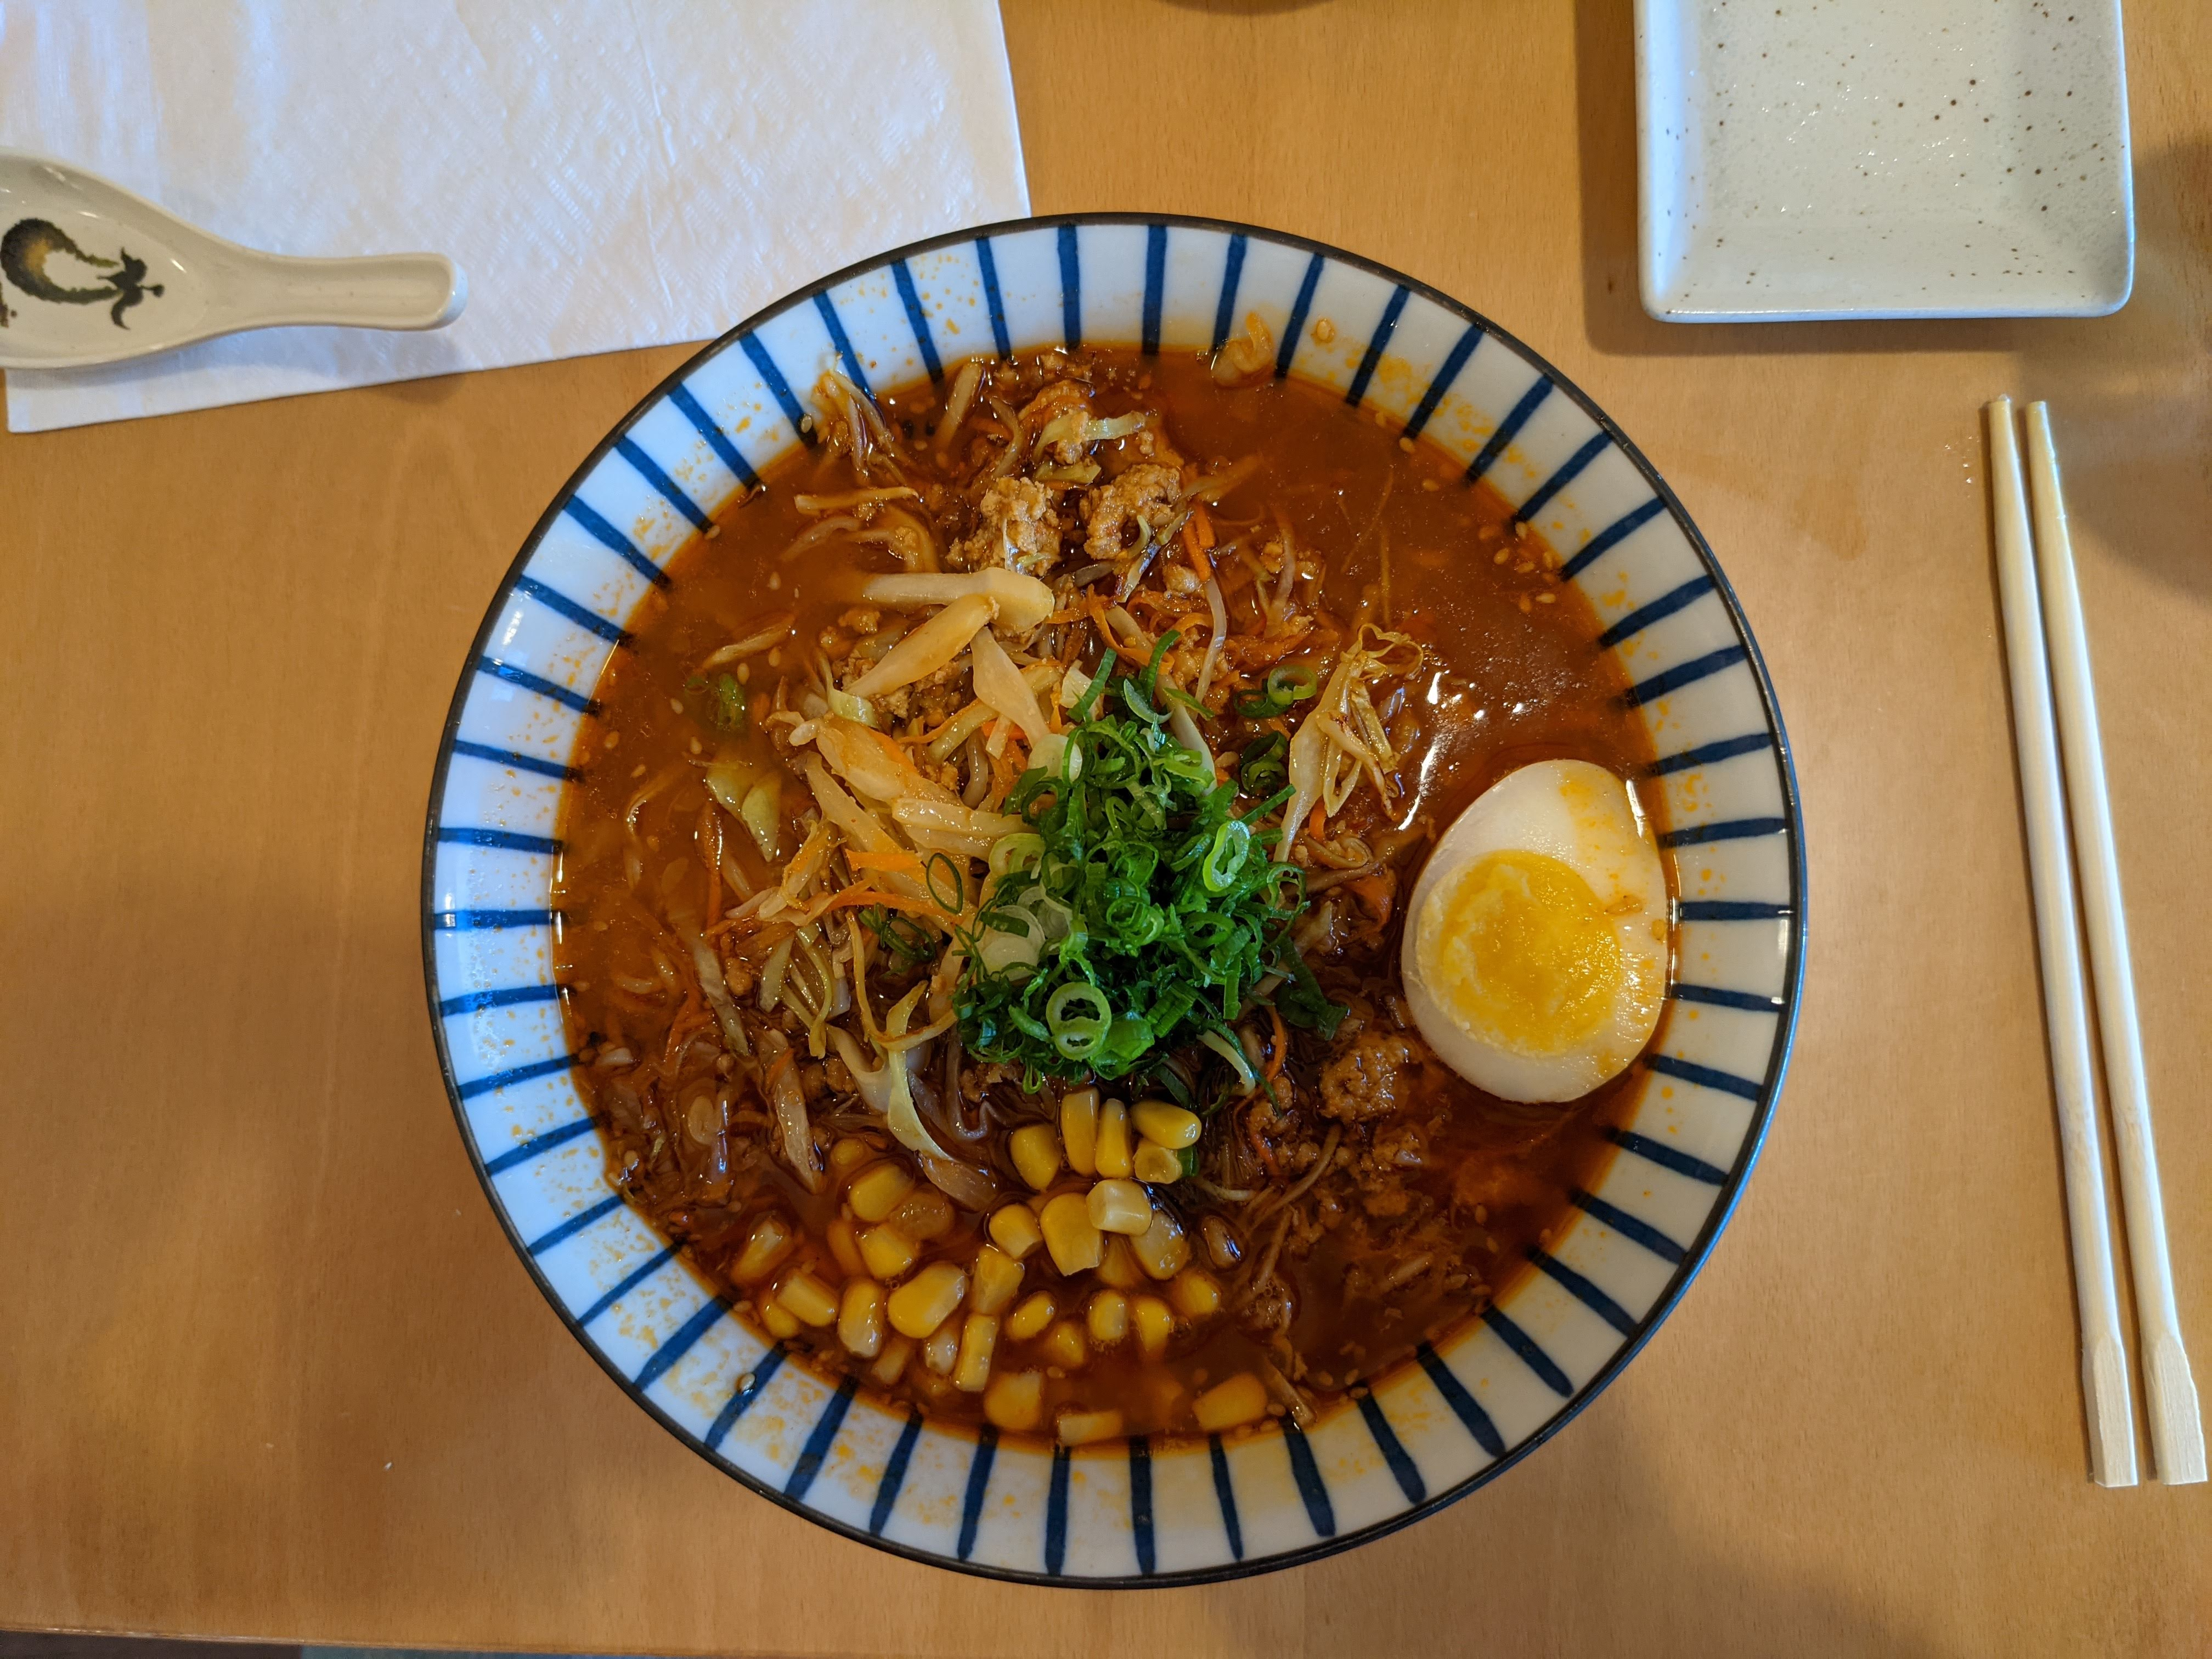
\includegraphics[width=.9\textwidth]{ramen1.jpg}
        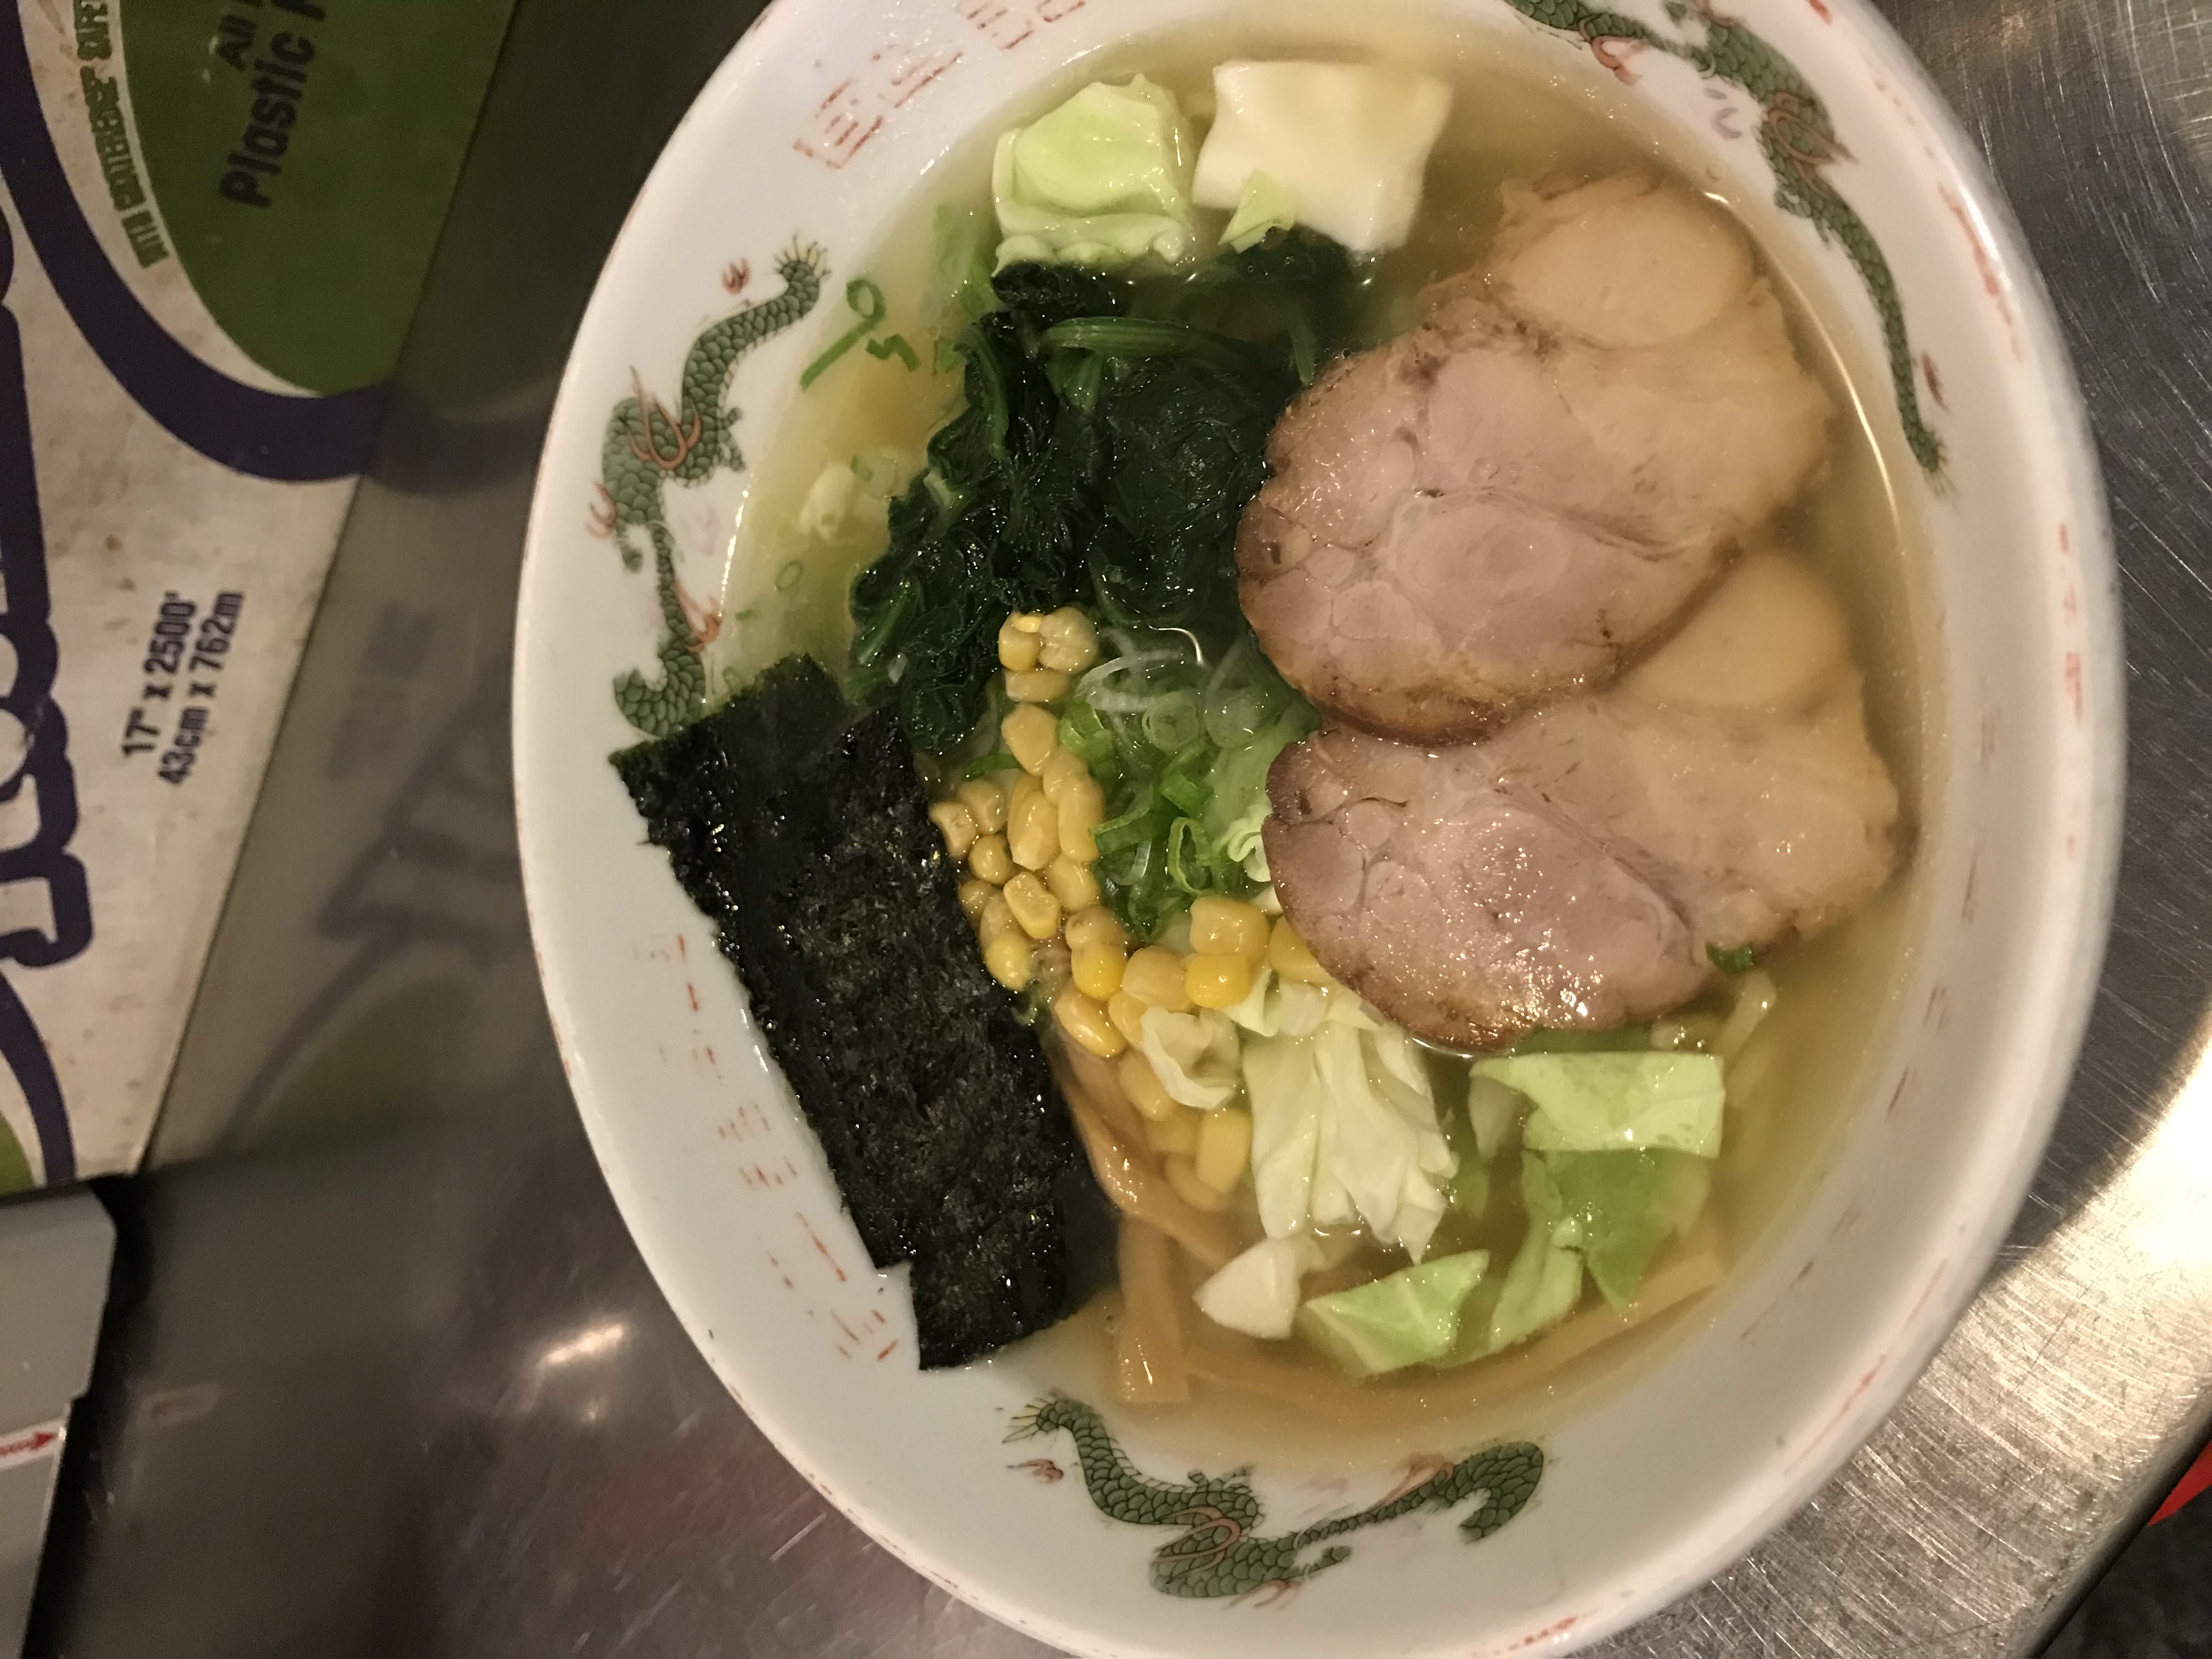
\includegraphics[width=.9\textwidth]{ramen2.jpg}
    \end{minipage}
\end{frame}

%%%%%%%%%%%%%%%%%%%%%%%%%%%%%%%%%%%%%%%
% Introduction
%%%%%%%%%%%%%%%%%%%%%%%%%%%%%%%%%%%%%%%
\section{Introduction}
\begin{frame}{Introduction}
    % Main topic
    \underline{Food Loss and Waste (FLW) happens everywhere.}
    % World trend
    \begin{itemize}
        \item One-third of food is lost or wasted around the world\cite{Gustavsson2011-em}.
        \item Around 1.3 billion tons of FLW is generated annually, and the rate is projected to grow by 44\% per year by 2025\cite{Blakeney2019-jk}.
    \end{itemize}
    % Canada 
    \begin{itemize}
        \item Canada creates about 35 million tons and the largest waste generator per capita in western countries in 2016\cite{Nzwc2016-jl}.
        \item Canada's avoidable FLW is \$49.5 million CAD\cite{Gooch2019-gd}.
    \end{itemize}
    % BC 
    \begin{itemize}
        \item In BC, 40\% of the waste to landfills is organic waste, the majority is produced from domestic waste\cite{BCwaste}.
    \end{itemize}
\end{frame}

% \subsection{Research}
\begin{frame}{Introduction}
    \underline{Few studies of FLW done on the supply side}
    \begin{itemize}
        \item Recent huge discoveries in the food waste research focus on waste generated by households:\cite{Aschemann-Witzel2015-xj,Lusk2017-xm,Von_Massow2019-qa}.
        % Nahman2012-ys,
    \end{itemize}

    \begin{itemize}
        \item Limited number of studies done on the food supply side.
        \item Even little estimations of FLW in food service industry.
        \item E.g. from 1.0\% to 15.5\% (up to 52\% under some conditions) \cite{Ministry_of_Environment_And_Climate_Change_Strategy2018-sk}. 
    \end{itemize}
\end{frame}

% \subsection{Research Questions}
\begin{frame}{Introduction}
    \begin{block}{Research Questions}
        \begin{itemize}
            \item What is the average volume of food that is wasted during processing and consumption in a restaurant?
            \item What is the extent of food wastage in Japanese restaurants in Prince George?
            \item What are the main factors contributing to food loss and waste?
            \item To what extent is a social or environmental impact from food loss and waste generated by a single restaurant?
            \item What approaches are Japanese restaurant operators taking to reduce food waste generation?
        \end{itemize}
    \end{block}
\end{frame}

%%%%%%%%%%%%%%%%%%%%%%%%%%%%%%%%%%%%%%%
% Literature Review
%% Definitions %%
%%%%%%%%%%%%%%%%%%%%%%%%%%%%%%%%%%%%%%%
\section{Literature Review}
\subsection{Definition}
\begin{frame}{Literature Review}
    \underline{What is Food Loss and Waste (FLW)?}
    \begin{block}{Definition of FLW (Source \cite{Ishangulyyev2019-uu})}
        \begin{table}[h]
            \begin{tabularx}{\textwidth}{l|X}
            \multicolumn{1}{c}{Organization} & \multicolumn{1}{c}{Definition} \\ \hline
                \small Food Loss (FAO)     
                & \footnotesize reduction in weight or quality of food for human consumption \\
                \small Food Waste (FAO)    
                & \footnotesize edible food discarded following spoilage or after the expiration date\\ \hline
                \small Food Waste (EU)     
                & \footnotesize any food removed from the food supply chain    \\ \hline
                \small Food Loss (US/CA)   
                & \footnotesize unused product from the food supply chain \\
                \small Food Waste (US/CA)  
                & \footnotesize still edible food scraps at disposal\\ \hline
                % \small Food Loss (HLPE)    
                % & \footnotesize decrease in food at the pre-consumer level, regardless of cause\\
                % \small Food Waste (HLPE)   
                % & \footnotesize food discarded at the consumer level\\ \hline
            \end{tabularx}
        \end{table}
    \end{block}
    $\implies$ No universally accepted definitions of FLW
\end{frame}

\begin{frame}{Literature Review}
     \begin{block}{Dim definition}
        \begin{itemize}
            \item Definition of FLW varies among organizations.
        \end{itemize}
        \begin{figure}
            \centering
            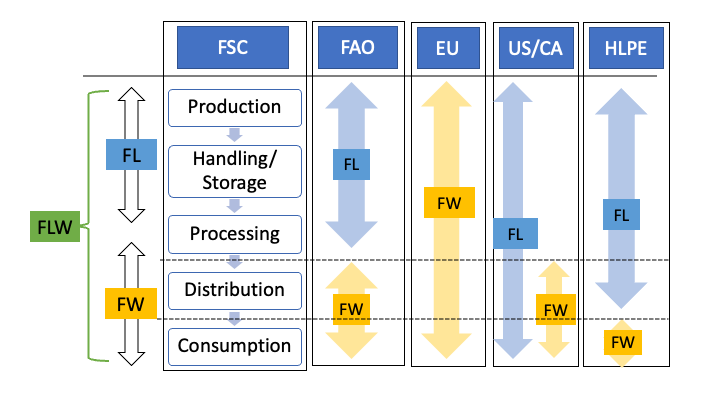
\includegraphics[width=0.7\textwidth,height=0.7\textheight,keepaspectratio]{defnFLW.png}
            %\caption{FLW Definitions}
        \end{figure}
     \end{block}
     \underline{General Idea:}
     \begin{itemize}
        \item Food Loss  $\Longleftrightarrow$ Upstream process.
        \item Food Waste $\Longleftrightarrow$ Downstream process.
    \end{itemize}  
\end{frame}


%% Liquid waste %%
\begin{frame}{Literature Review}
    \underline{Few studies on liquid food waste}
    
    \begin{block}{Not only Solid but Liquid food}       
        \begin{itemize}
            \item All these-above defined FLW are solid waste
            \item e.g. food scraps, peels, or leftovers
            \item Not only solid but also liquid waste
            \item Environmental pollutions: soil, water, and air contamination
            \item Drainage blockages: clog drains and sewage blockages
            \item Resource Losses: water, energy, land used to produce food
        \end{itemize}
    \end{block}
\end{frame}

\begin{frame}{Literature Review}
    \underline{In this research on a restaurant's FLW:}
    \begin{block}{Definition of FLW in Restaurant}
        \begin{itemize}
            \item Food Loss: generated by \textbf{provider}
            \item Food Waste: generated by \textbf{consumers}
            \begin{itemize}
                \item Solid Food Waste: solid portion of food waste
                \item Liquid Food Waste: liquid portion of food waste
            \end{itemize}
        \end{itemize}
    \end{block}
        \begin{figure}
            \centering
            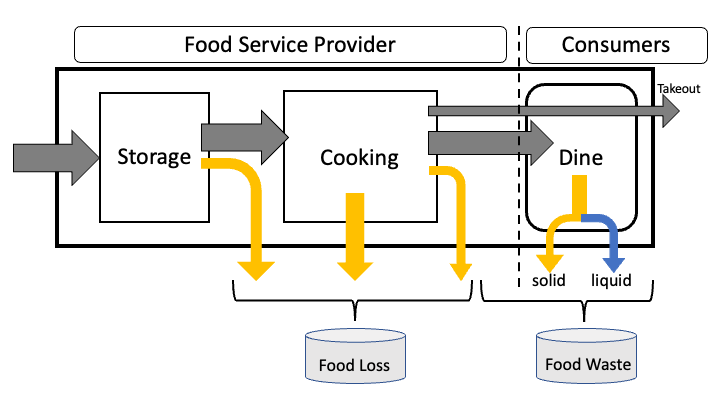
\includegraphics[width=0.7\textwidth,height=0.7\textheight,keepaspectratio]{defnFLWrest.png}
            %\caption{Flow of FLW}
        \end{figure}
\end{frame}

%%%%%%%%%%%%%%%%%%%%%%%%%%%%%%%%%%%%%%%
% Literature Review
%% Measurements %%
%%%%%%%%%%%%%%%%%%%%%%%%%%%%%%%%%%%%%%%
\subsection{Measurements}
\begin{frame}{Literature Review}
    \underline{How to measure FLW?}
    \begin{block}{FLW Measurements used in the past research}
    \begin{table}[]
        \begin{tabular}{ll}
            \hline
            \multicolumn{1}{c}{Method} & \multicolumn{1}{c}{Note}            \\ \hline
                1. \small Self-report   & \footnotesize individuals report FLW                    \\
                                 & \footnotesize low-cost but high dropouts                \\
                2. \small Survey        & \footnotesize collect FLW by interview or questionnaire \\
                                 & \footnotesize cost-effective but not accurate           \\
                3. \small Composition   & \footnotesize sample and analysis at lab                \\
                                 & \footnotesize need special knowledge and equipment      \\
                4. \small Mass balance  & \footnotesize material flow analysis                    \\
                                 & \footnotesize limitation in waste factor assumptions    \\
                5. \textbf{\small Direct weight} 
                                 & \footnotesize directly measure FLW                      \\
                                 & \footnotesize most accurate but high cost         \\ \hline
        \end{tabular}
    \end{table}
    \end{block}
\end{frame}

%%%%%%%%%%%%%%%%%%%%%%%%%%%%%%%%%%%%%%%
% Literature Review
%% Potential Factors %%
%%%%%%%%%%%%%%%%%%%%%%%%%%%%%%%%%%%%%%%
\subsection{Potential Factors}
\begin{frame}{Literature Review}
    % \begin{itemize}
    %     \item Mysterious factors of FLW.
    % \end{itemize}
    \underline{What is the main factors of FLW?}
    \begin{block}{8 Classifications (\cite{Heikkila2016-el})}
        \begin{enumerate}
            \item \textbf{Society}: \small culture, awareness and legislation.
            \item \textbf{Business model}: \small a la carte or buffet style.
            \item \textbf{Product procurement}: \small raw or frozen; where to buy.
            \item \textbf{Management}: \small menu development, inventories.
            \item \textbf{Professional skills}: \small untrained mistakes throwing food.
            \item \textbf{Diners}: \small preference, taste or presentation mismatch.
            \item \textbf{Competitors}: \small existence of other restaurants.
            \item \textbf{Communication}: \small with customers and with staff.
        \end{enumerate}
    \end{block}
    $\implies$ No substantial change during the study period.
\end{frame}

\begin{frame}{Literature Review}
    \underline{Any other potential factors of FLW?}
    % Due to the short-term sample collection,
    \begin{block}{Other factors}
        \begin{itemize}
            \item \textbf{Calendar effect}: sales varys between months, day of week, holidays.
            \item \textbf{Weather coditons}: ice cream salls well in summer and not in winter.
        \end{itemize}       
    \end{block}
    $\implies$ Calendar effect (week of the day) and weather conditions (temperature, humidity, precipitation) may cause FLW?
\end{frame}

%%%%%%%%%%%%%%%%%%%%%%%%%%%%%%%%%%%%%%%
% Literature Review
%% Stat model %%
%%%%%%%%%%%%%%%%%%%%%%%%%%%%%%%%%%%%%%%
\subsection{Statistical Model}
\begin{frame}{Literature Review}
    \underline{How to test associations between FLW and potential factors?}
    \begin{block}{Regression Model and Strategy}
        \centering$Y = X\beta + \epsilon$\\
        \begin{itemize}
            \item set-up regression model
            \item test whether true slopes $\beta$ is zero or not
        \end{itemize}
    \end{block}
    where,\\
        $Y$ is \{daily food waste, liquid waste, solid waste\},\\
        $X$ is \{temperature, humidity, precipitation, day of week, \#customers, sales, liquors\}.
\end{frame}

% \begin{frame}{Literature Review}
%     \underline{Regression analysis on time series might arise a problem.}
%     \begin{block}{Linear Regression Model and Assumptions}
%         \centering $Y = X\beta + \epsilon$\\
%         \centering $\epsilon \overset{\text{i.i.d.}}{\sim} N(0, \sigma^2)$
%         \small
%         \begin{tabular}{ll}
%             \hline
%             \multicolumn{1}{c}{Assumption} & \multicolumn{1}{c}{Problem}    \\ \hline
%             1. $\mathop{\mathbb{E}}(\epsilon) = 0.$ & may have trend  \\
%             2. $Var(\epsilon) = \sigma^2.$& heterocedascity                \\
%             3. $Cov(\epsilon_i,\epsilon_j) = 0, i\neq j.$& autocorrelation b/w 2 pts \\
%             4. $X \independent \epsilon$ and no R.V. $X$ & a point of x influences y      \\
%             5. $\epsilon$ follows Normal dist'n & (other distribution)           \\
%             6. Linearly independent of $X$ & (multicolinearlity)            \\ \hline
%             \end{tabular}  
%     \end{block}   
%     $\implies$ \textbf{spurious regression}: a conclusion is that an association exists between two variables even though there is no relationship between them at all.
% \end{frame}

% \begin{frame}{Literature Review}
%     \begin{itemize}
%         \item Create fake two data sets without no association
%         \begin{enumerate}
%             \item[1.] simply random select
%             \item[2.] dependent on one before (random-walk)
%         \end{enumerate}
%         \item Check the relationship between two data
%     \end{itemize}
%     \begin{block}{Spurious regression}
%     \centering
%         \begin{tabular}{cc}
%             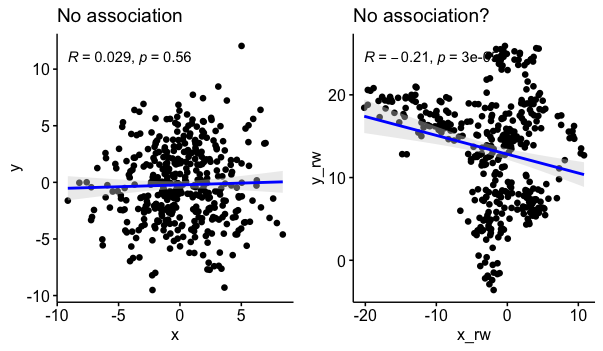
\includegraphics[width=4.5cm]{spuriousRegression.png}
%                     &
%             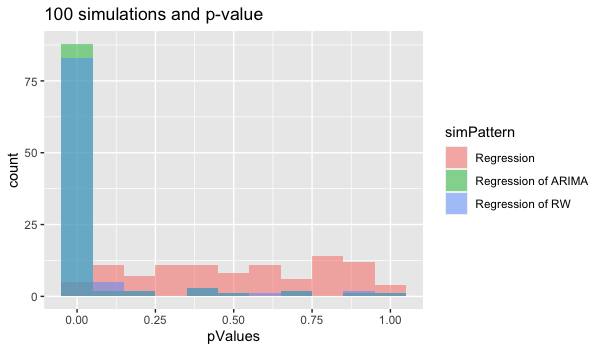
\includegraphics[width=4.5cm]{100pvalues.png}\\
%         \end{tabular}
%     \end{block}
%     $\implies$ If random-walk process, usual regression analysis may achieve false results.
% \end{frame}


% \begin{frame}{Literature Review}
%     \begin{block}{Dynamic Regression Modelling}
%         \underline{time-vary coefficients parameter $\beta$}
%         \small
%         \begin{tabular}{l p{4cm}} 
%                 \begin{array}[b]{l}
%                      y_i \sim \text{N}(\mu_i, \sigma_y^2),\\
%                      \mu_i = X\beta_i\footnote{$\mu_i = a_i + b_i * x_i$},\\
%                      \beta_i \sim \text{N}(\beta_{i-1}, \sigma_\beta^2), \forall i \in T.\\   
%                 \end{array}
%                 &
%                 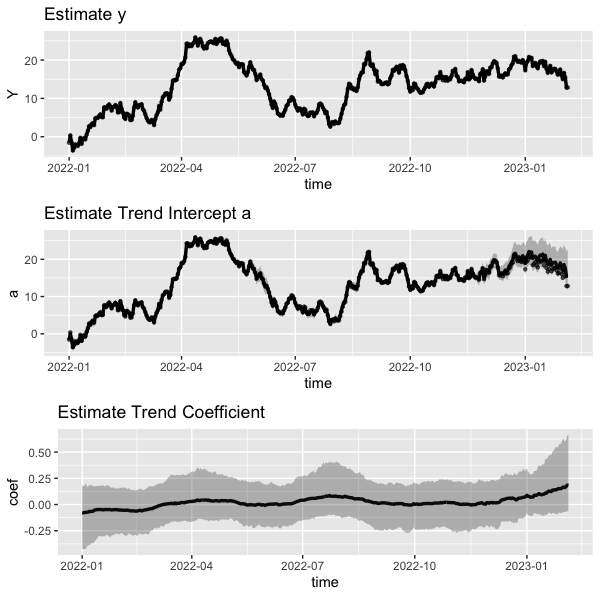
\includegraphics[keepaspectratio=true,width=.4\paperwidth,valign=c]{bayesianModel_rw.png}
%         \end{tabular}     
%     \end{block}
% \end{frame}

%%%%%%%%%%%%%%%%%%%%%%%%%%%%%%%%%%%%%%%
% Literature Review
%% Effects of FLW %%
%%%%%%%%%%%%%%%%%%%%%%%%%%%%%%%%%%%%%%%
\subsection{Effects of FLW}
\begin{frame}{Literature Review}
    \underline{What is the consequence of FLW?}
    \begin{block}{Effects of FLW}
        \begin{itemize}
            \item \textbf{Economic Loss}:\\
             loss of resources: labour, material, time, and energy
            \item \textbf{Environmental Effects}:\\
            water pollution, deforestation, soil erosion, and GHG
            \item \textbf{Social Impacts}: food insecurity and social inequality\\    
        \end{itemize}
    \end{block}

Reducing FLW can mitigate these economic and environmental impacts.
Through better supply chain management, reducing consumer food waste,
and increasing food recovery.

\end{frame}

%%%%%%%%%%%%%%%%%%%%%%%%%%%%%%%%%%%%%%%
% Literature Review
%% Research Goals %%
%%%%%%%%%%%%%%%%%%%%%%%%%%%%%%%%%%%%%%%
\subsection{Hypothesis}
\begin{frame}{Literature Review}
    \begin{block}{Research Goals}
        \begin{itemize}
            \item Estimate average FLW
            \item Any patterns between FLW and business operations
            \item Any association between FLW and weather conditions
            \item Estimate economic and environmental impacts
        \end{itemize}
    \end{block}
\end{frame}

%%%%%%%%%%%%%%%%%%%%%%%%%%%%%%%%%%%%%%%
% Methods
%% Study Area %%
%%%%%%%%%%%%%%%%%%%%%%%%%%%%%%%%%%%%%%%
\section{Methods}
\subsection{Study Area}
\begin{frame}{Methods}
    \underline{Which restaurant is to be studied?}
    \begin{block}{Study Area}
        \begin{itemize}
            \small
            \item \textbf{Location}: Japanese restaurant (suburban area of PG)
            \item \textbf{Hours}: lunch and dinner for three hours each
            \item \textbf{Day}: six days of a week (Tue to Sun; Mon closed)
            \item \textbf{Offer}: dine-in \& takeouts
            \item \textbf{Items}: sushi \& \underline{ramen} (soup and noodle)
            \item \textbf{Duration}: 6-month (Sept. to Mar.)
            \item \underline{\textbf{Permission}}: 
            \checkbox{1} Cooperation; \checkbox{0} Name disclosure.
        \end{itemize}
    \end{block}
        \begin{figure}
            \centering
            \subfloat{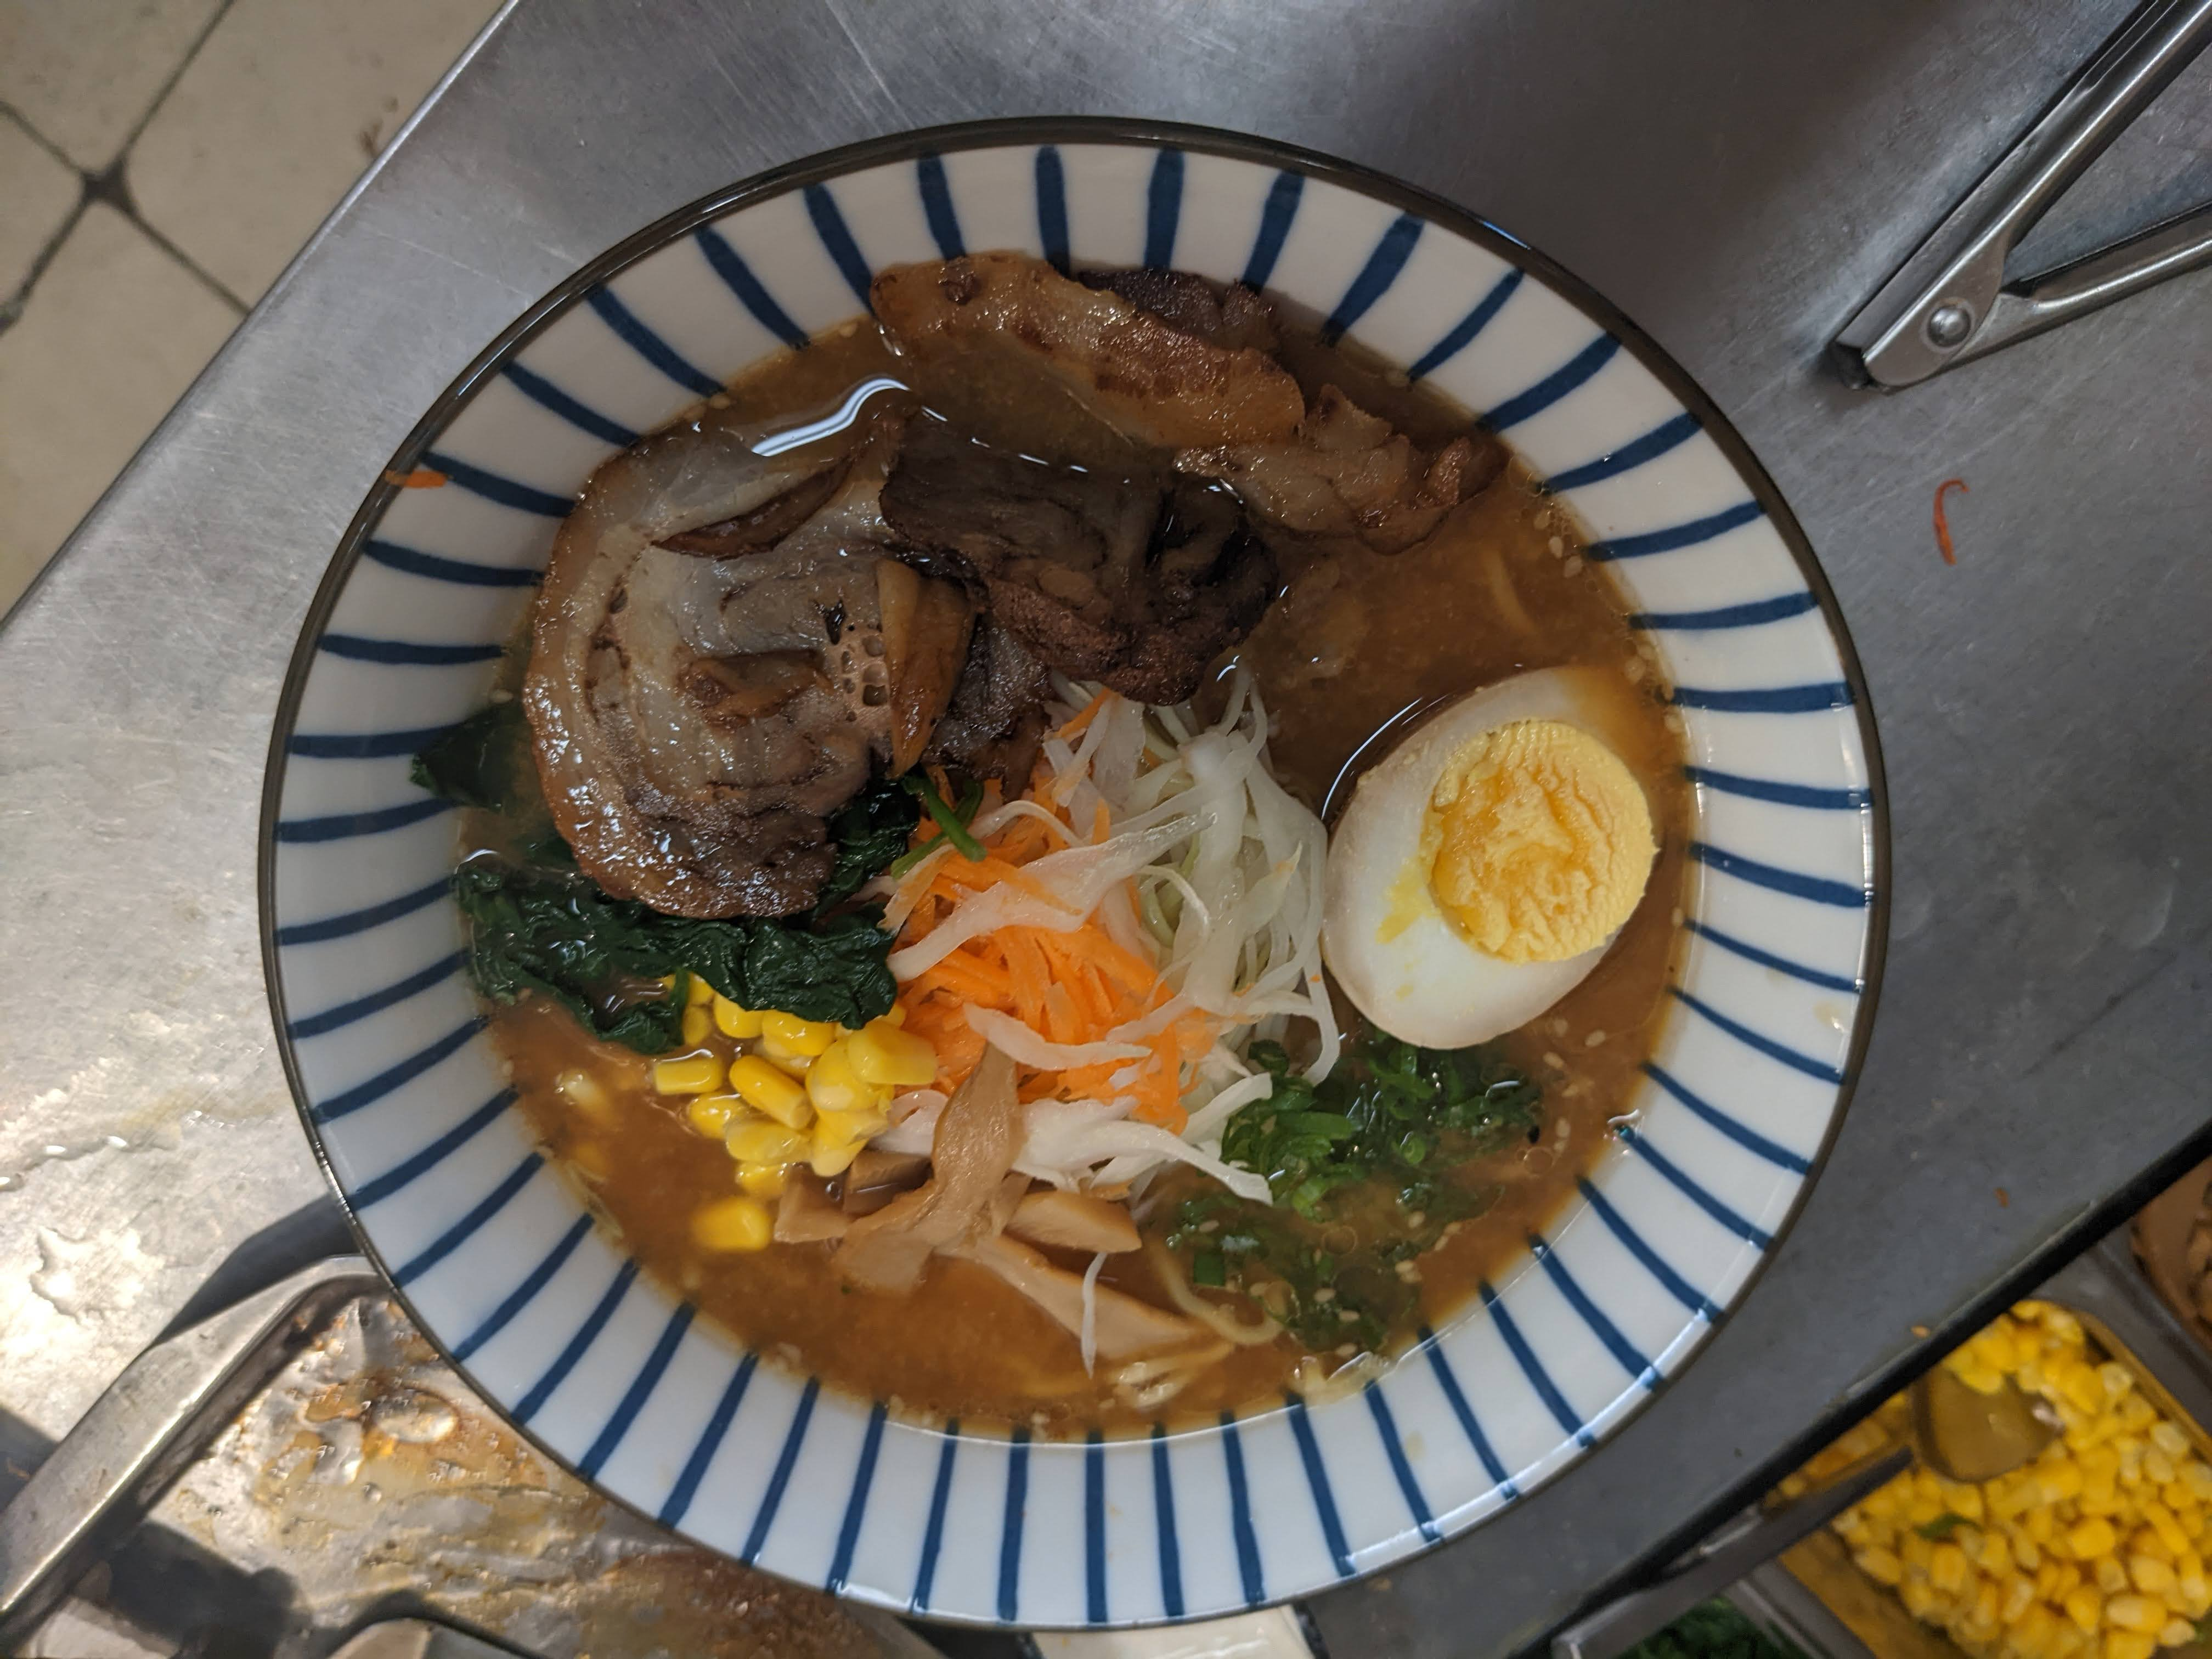
\includegraphics[width=2.5cm]{ramen.jpg}}%
            \qquad
            \subfloat{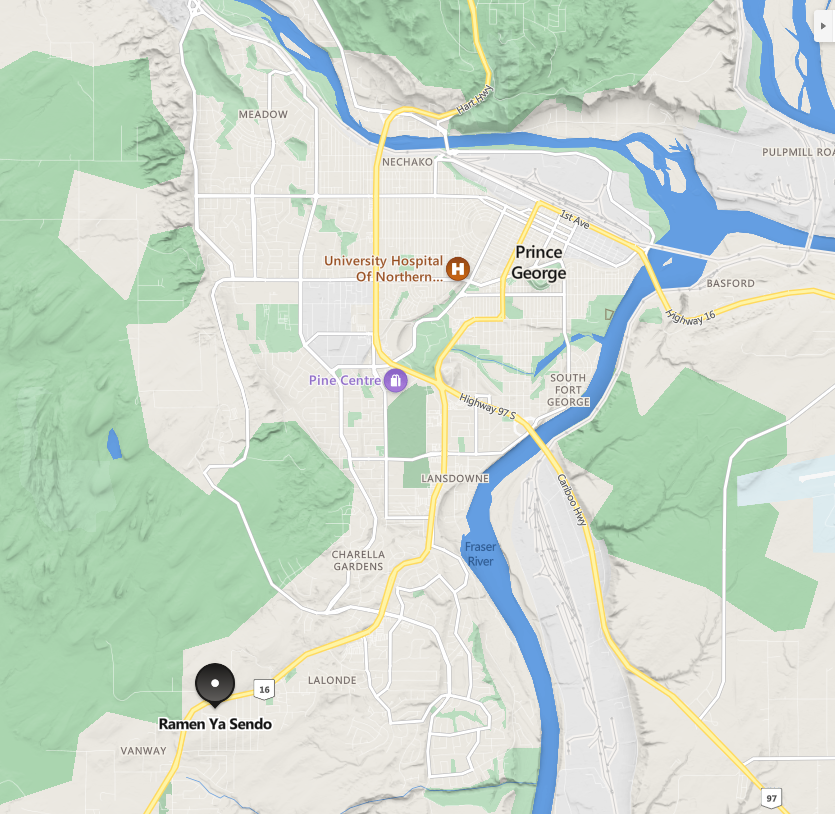
\includegraphics[width=2cm]{sendoMap.png}}%
            \caption{Research Location Site}
        \end{figure}
\end{frame}

%%%%%%%%%%%%%%%%%%%%%%%%%%%%%%%%%%%%%%%
% Methods
%% Apparatus %%
%%%%%%%%%%%%%%%%%%%%%%%%%%%%%%%%%%%%%%%
\subsection{Apparatus}
\begin{frame}{Methods}
    \underline{How to capture the FLW?}
    \begin{block}{Collection Apparatus}
        % \begin{table}[]
            \begin{tabular}{cc}
                    Bucket for FL & Bucket \& Colander for FW \\ \hline
                    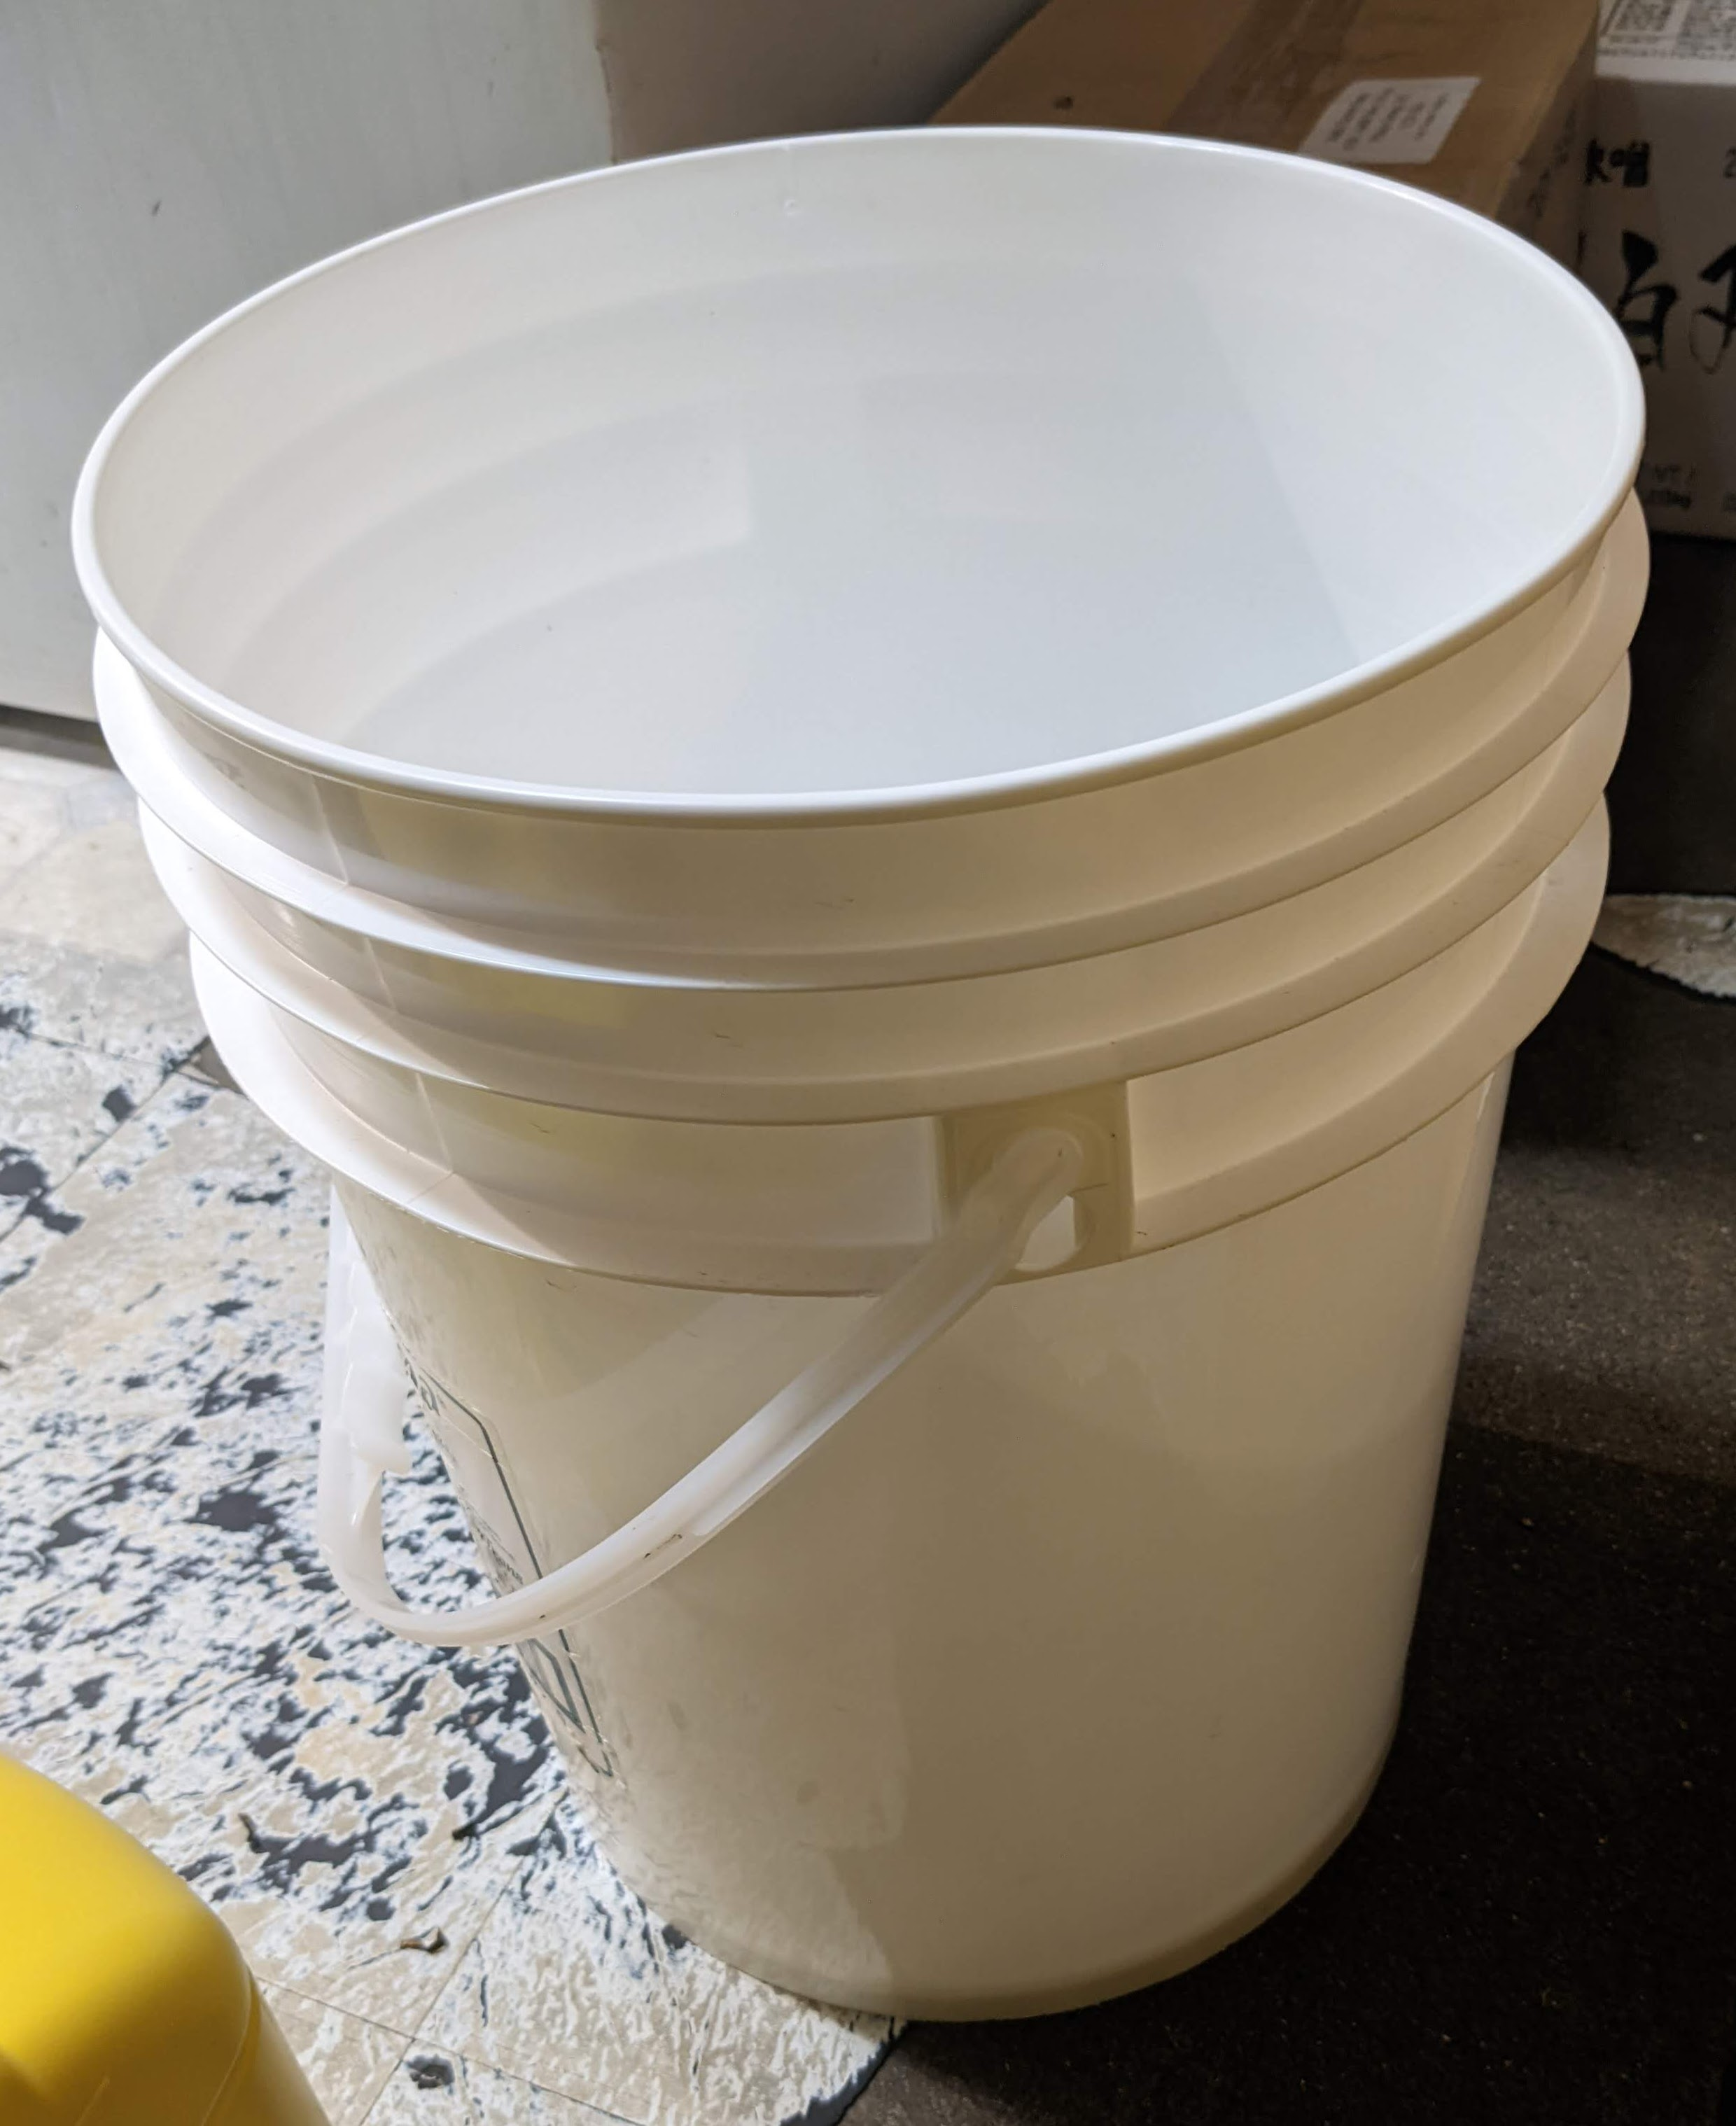
\includegraphics[width=1.7cm]{busket.jpg}
                    & 
                    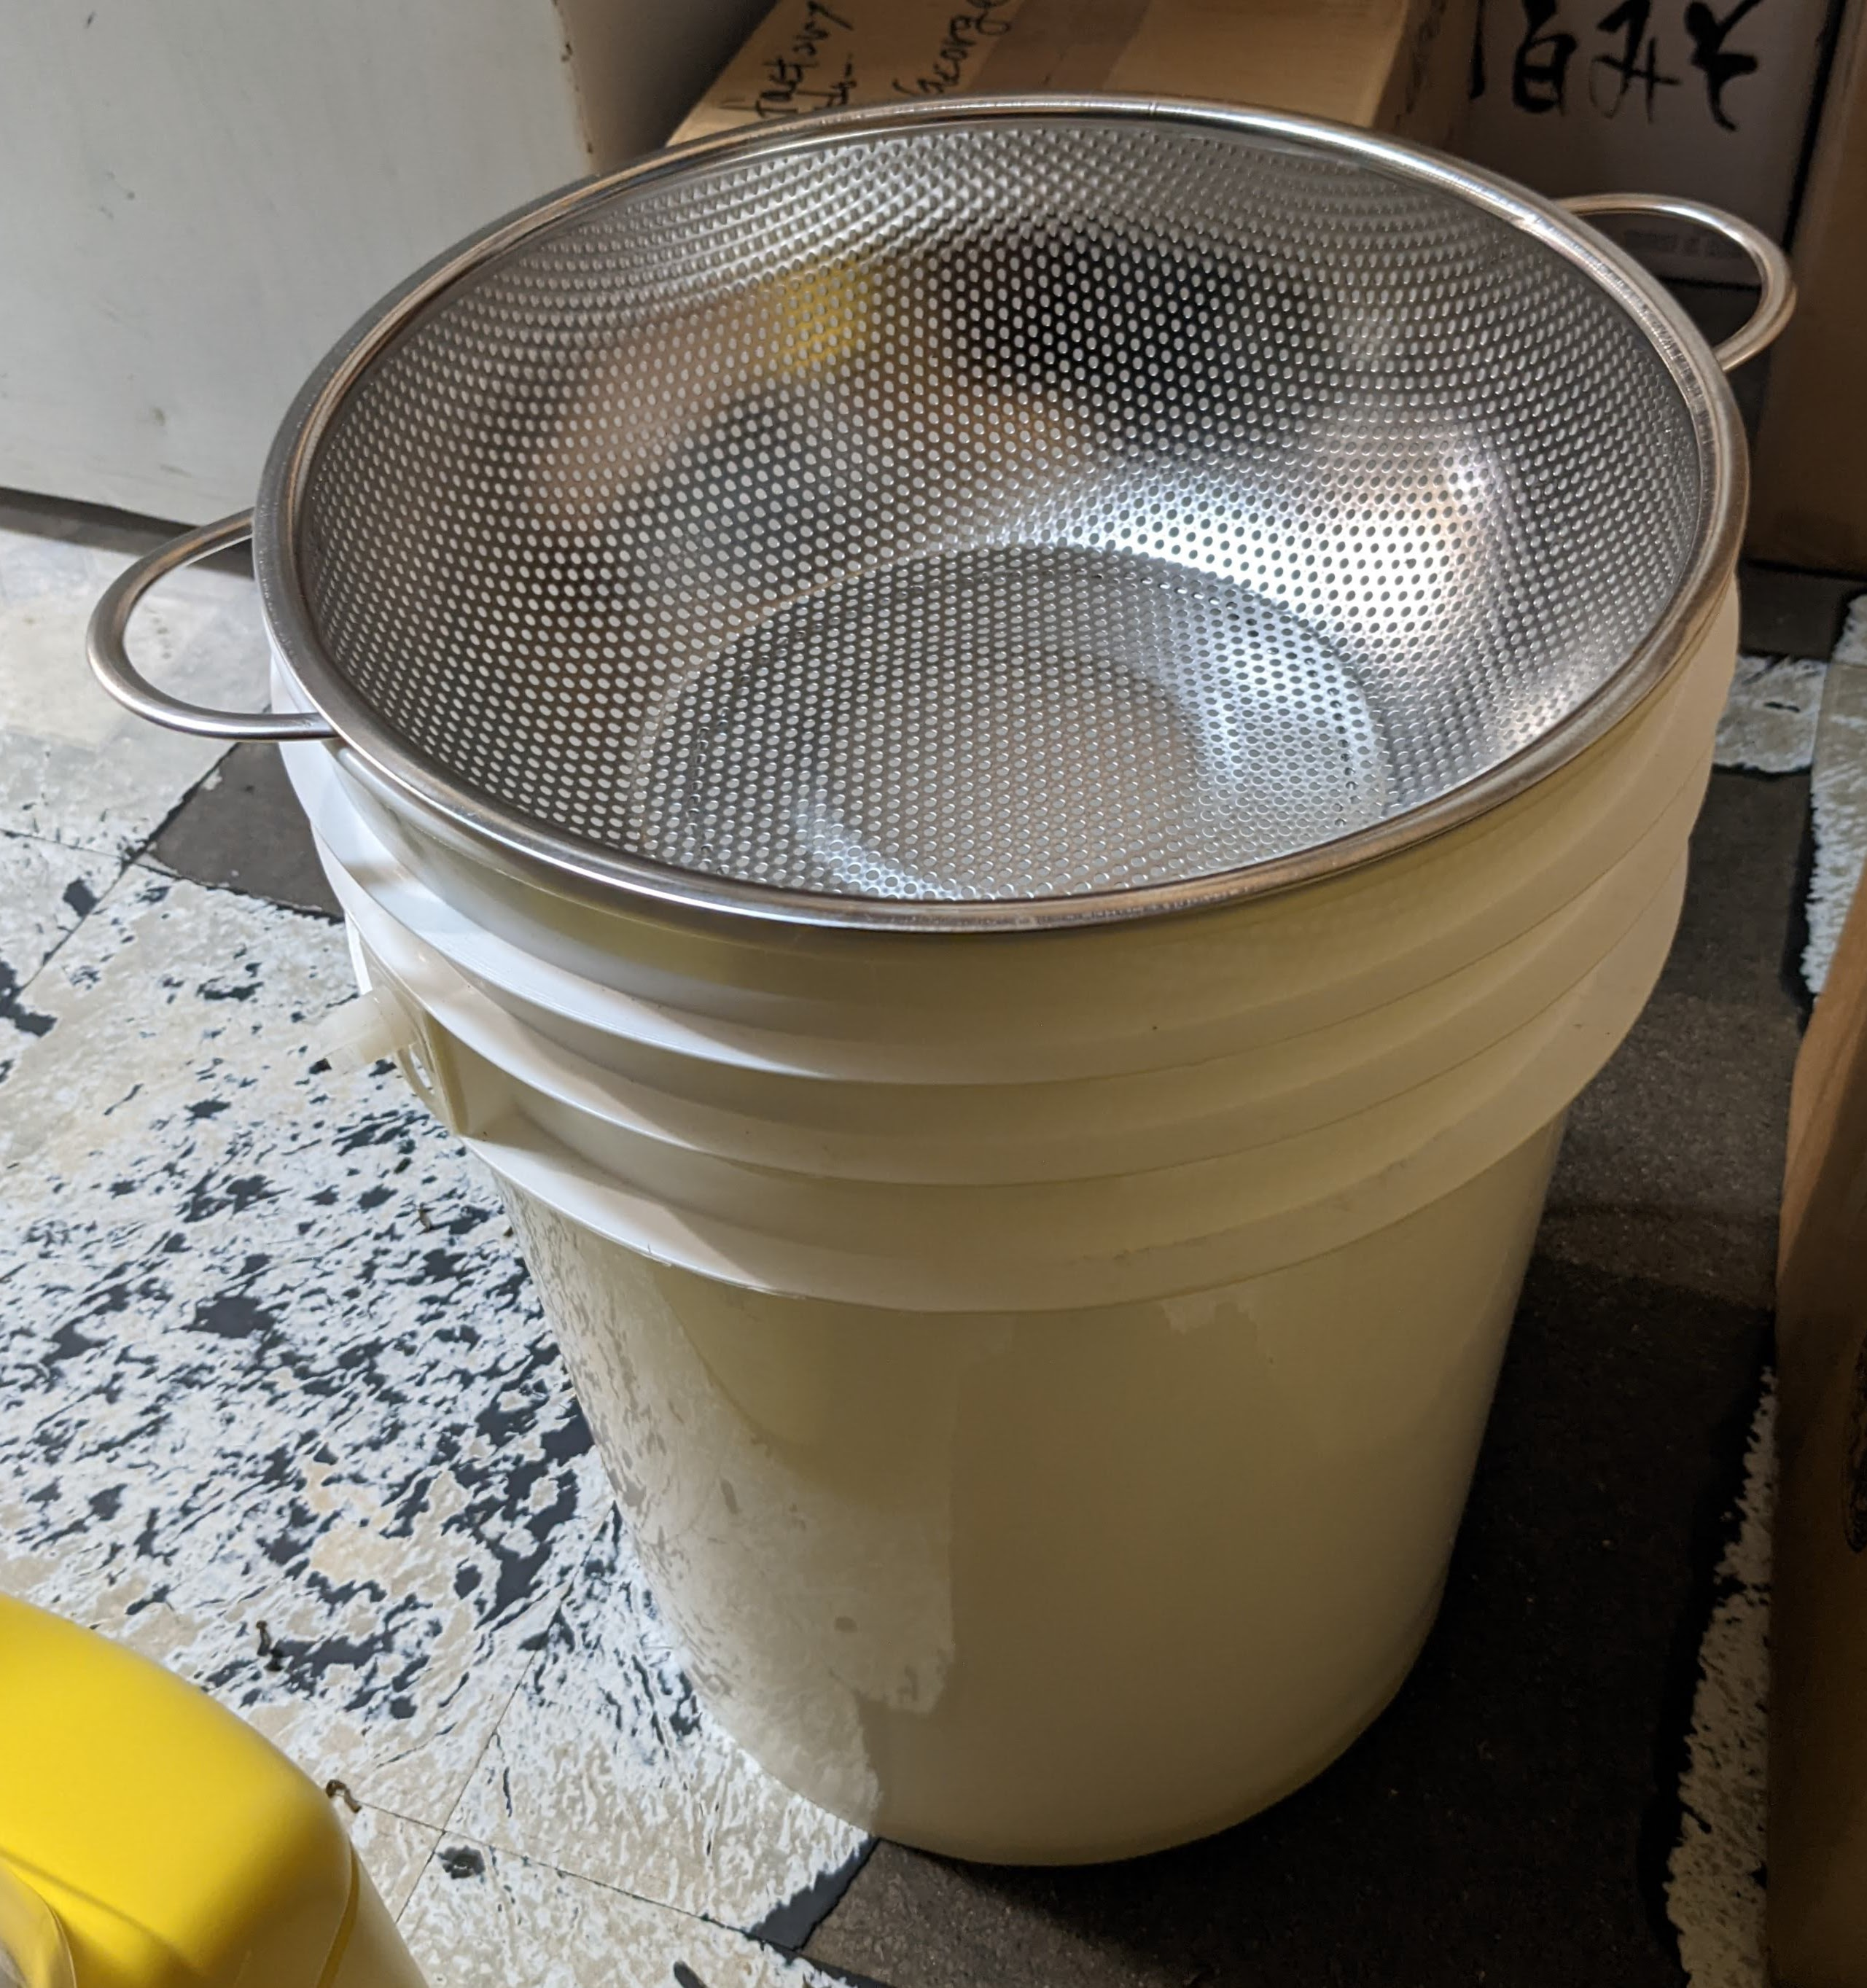
\includegraphics[width=1.8cm]{busketStrainer.jpg}\\
                    % \hline
                    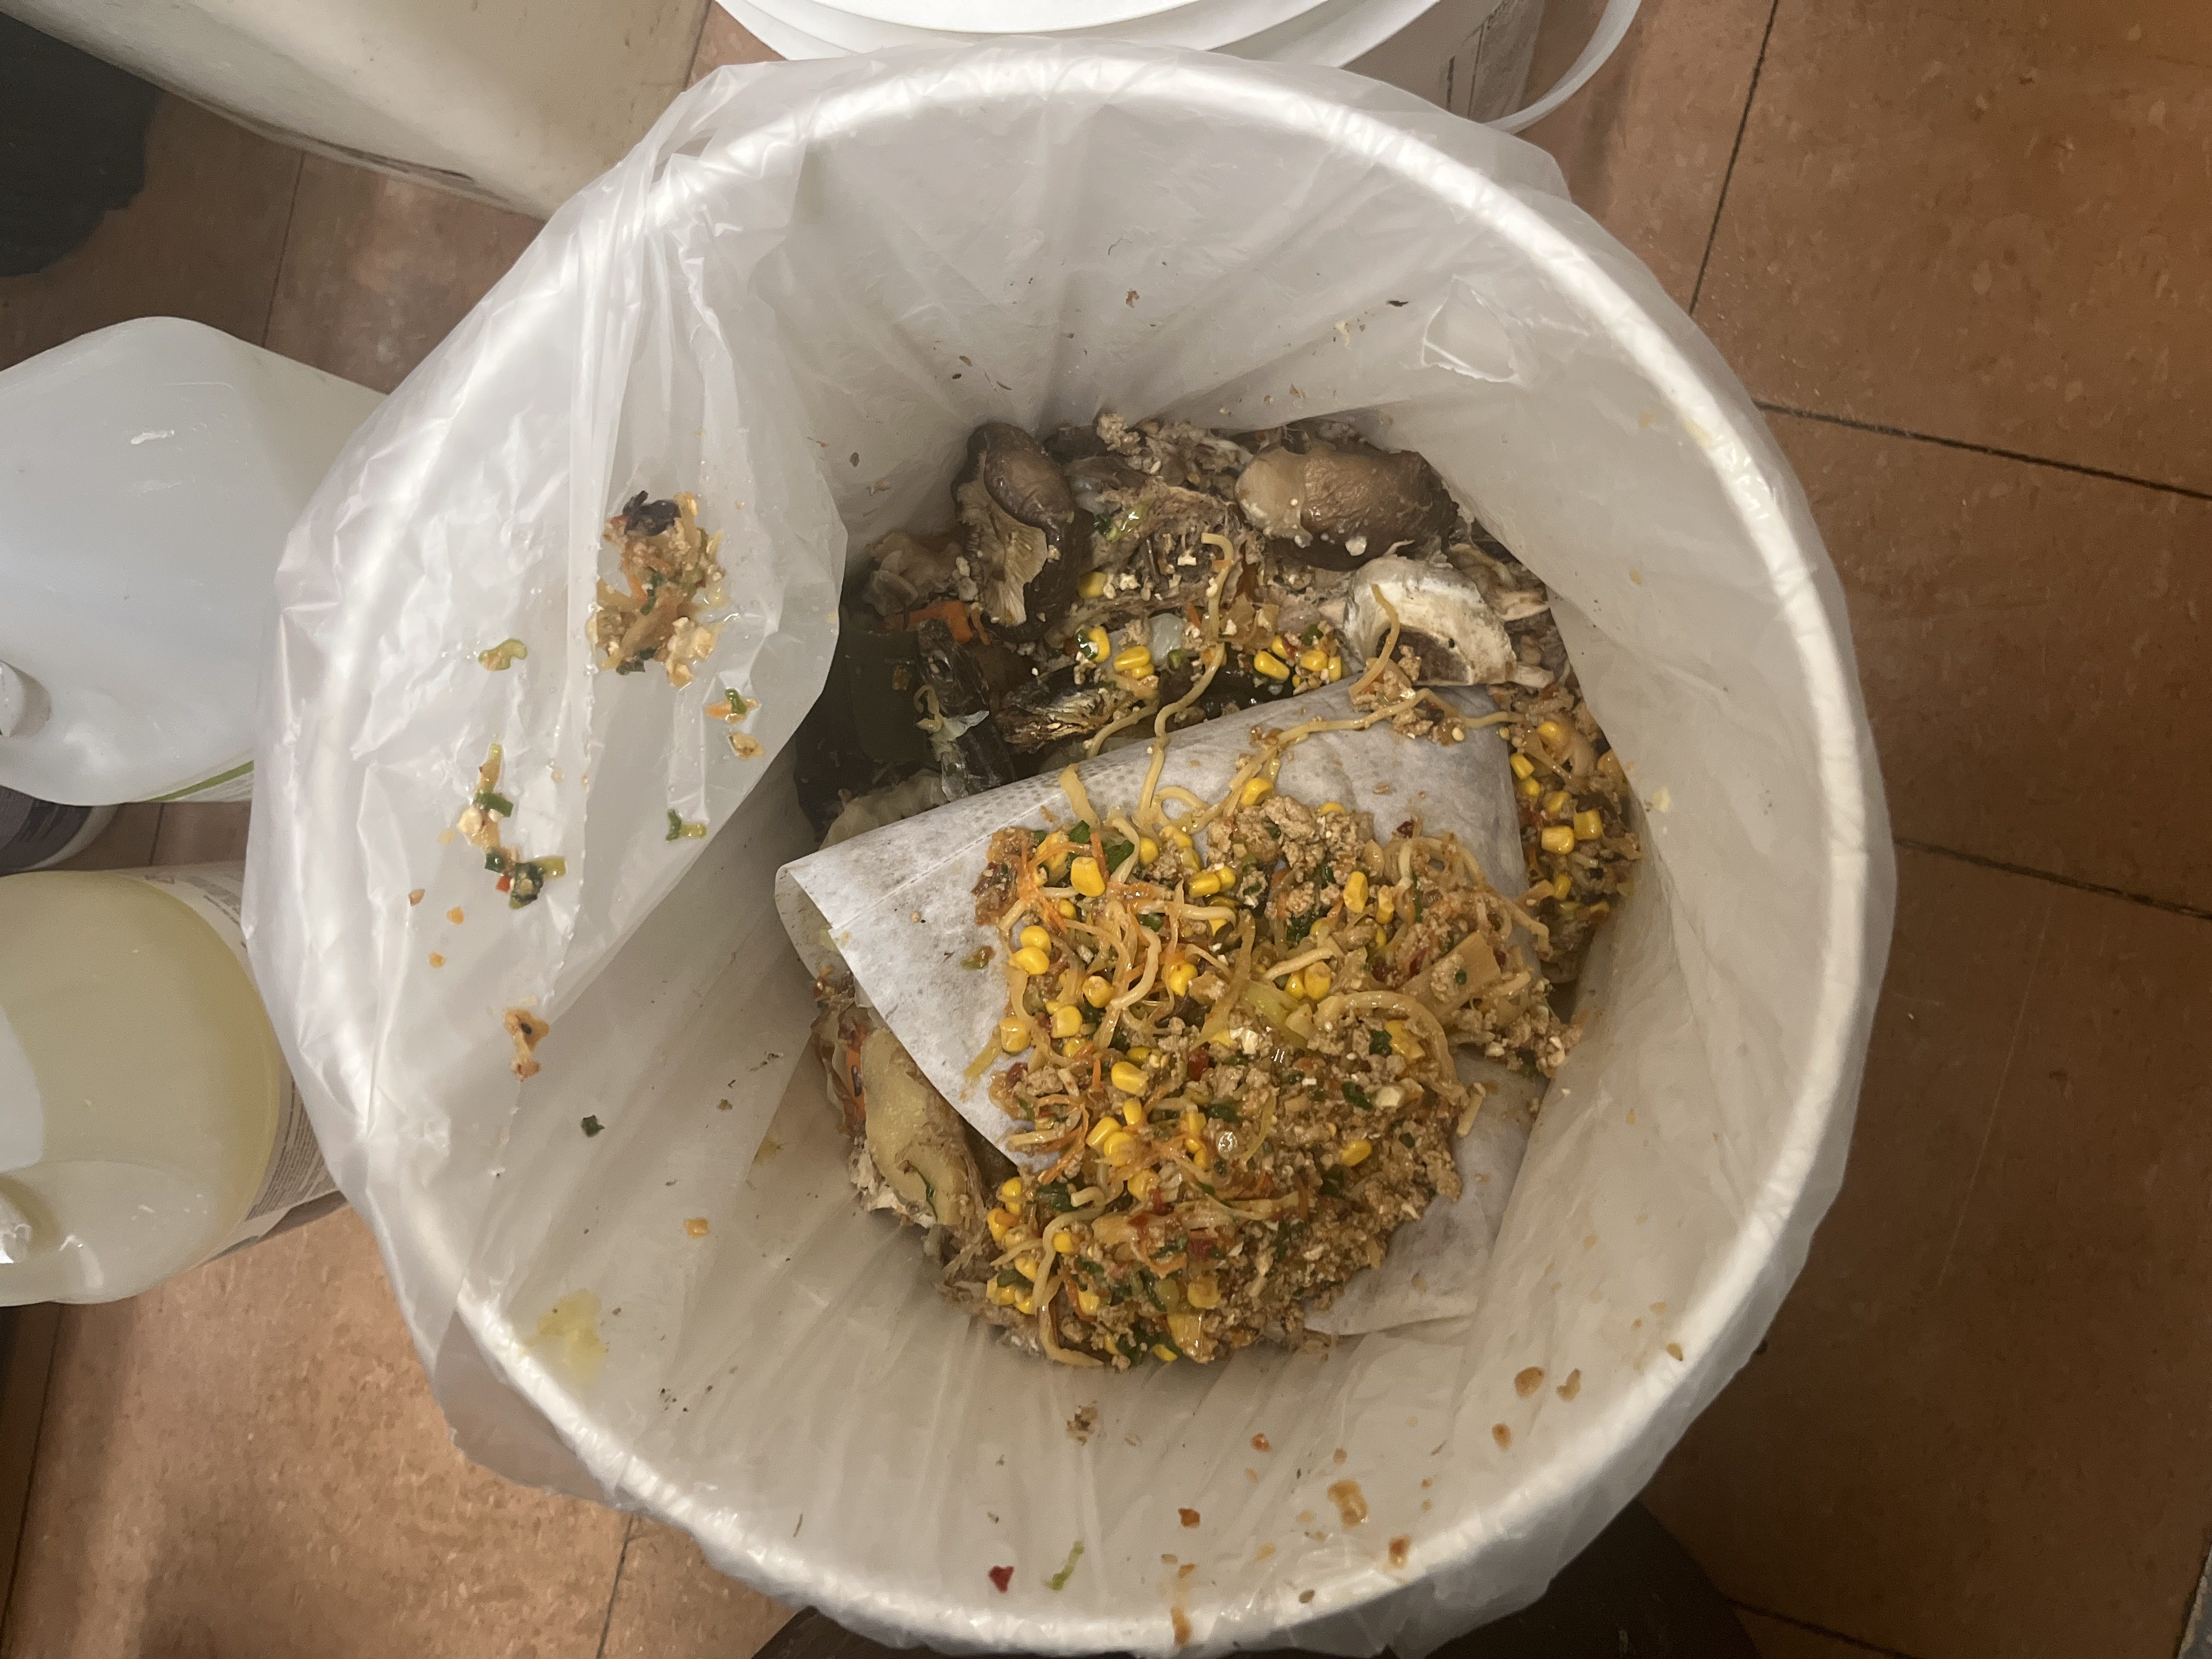
\includegraphics[width=1.7cm]{fl.jpg}
                    & 
                    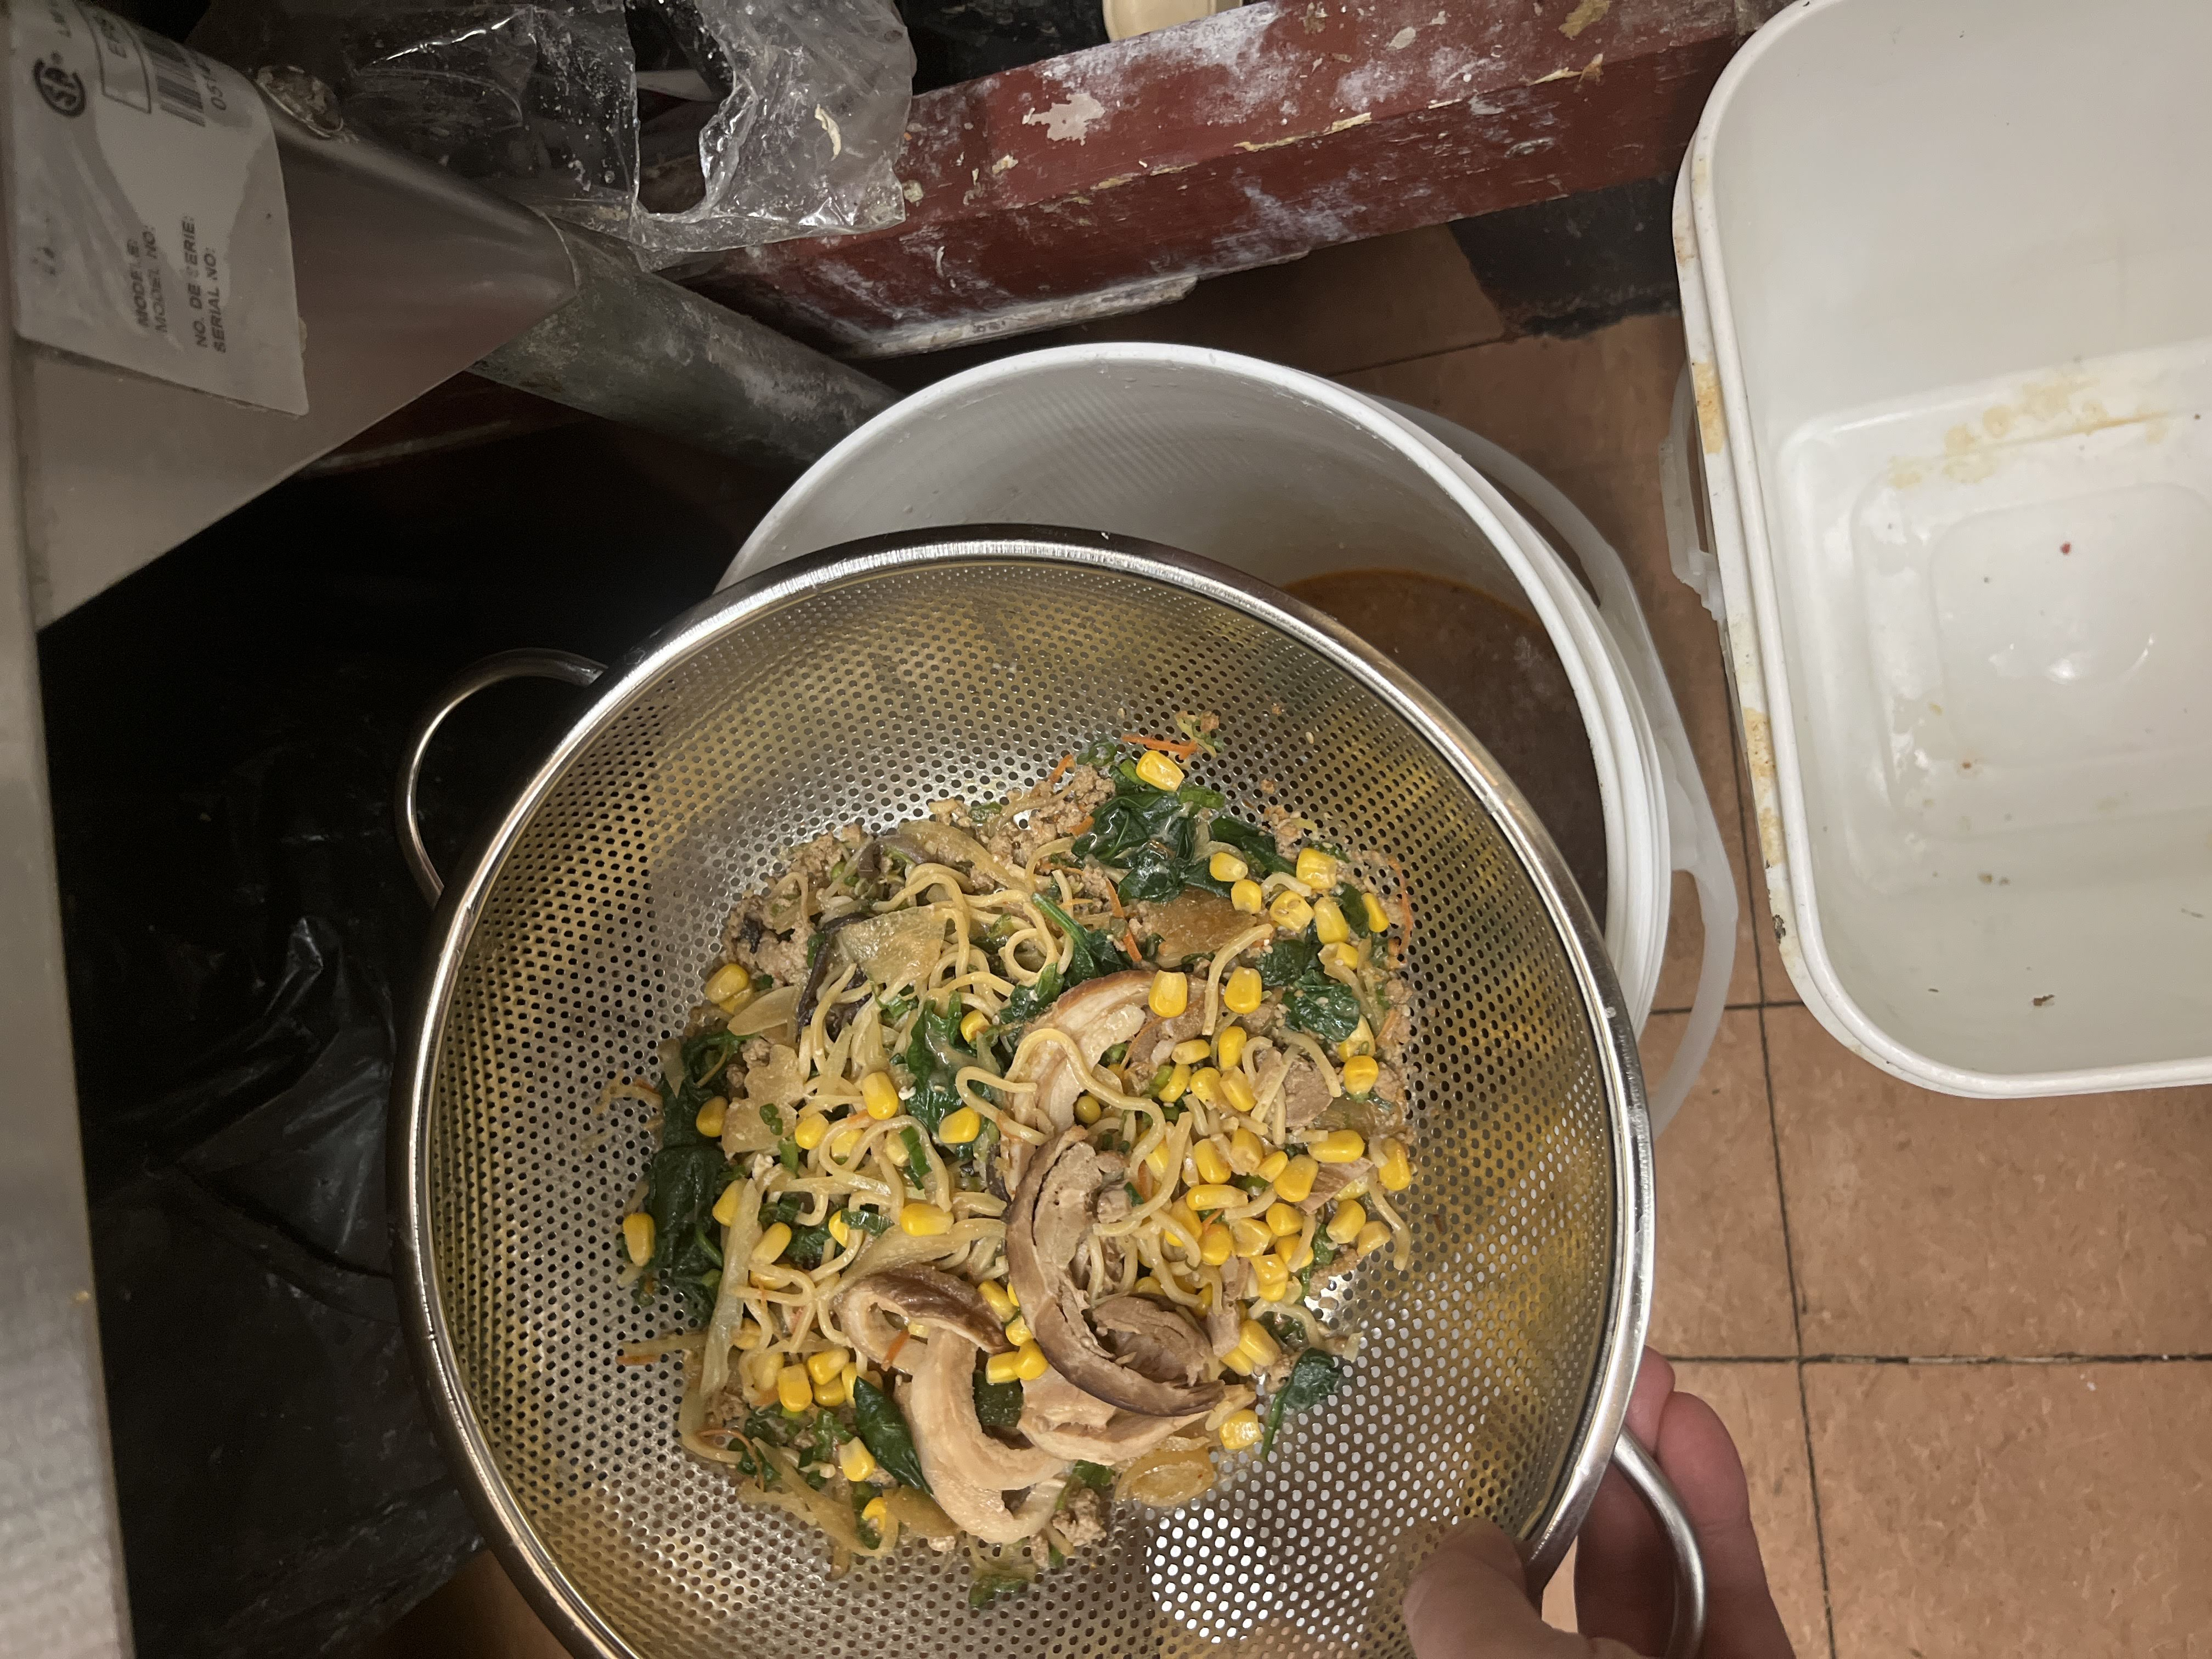
\includegraphics[width=1.8cm]{leftovers.jpg}\\
                    \hline
                    Weight scale (0.05 - 150 kg) & Pen \& notebook\\ %\hline
                    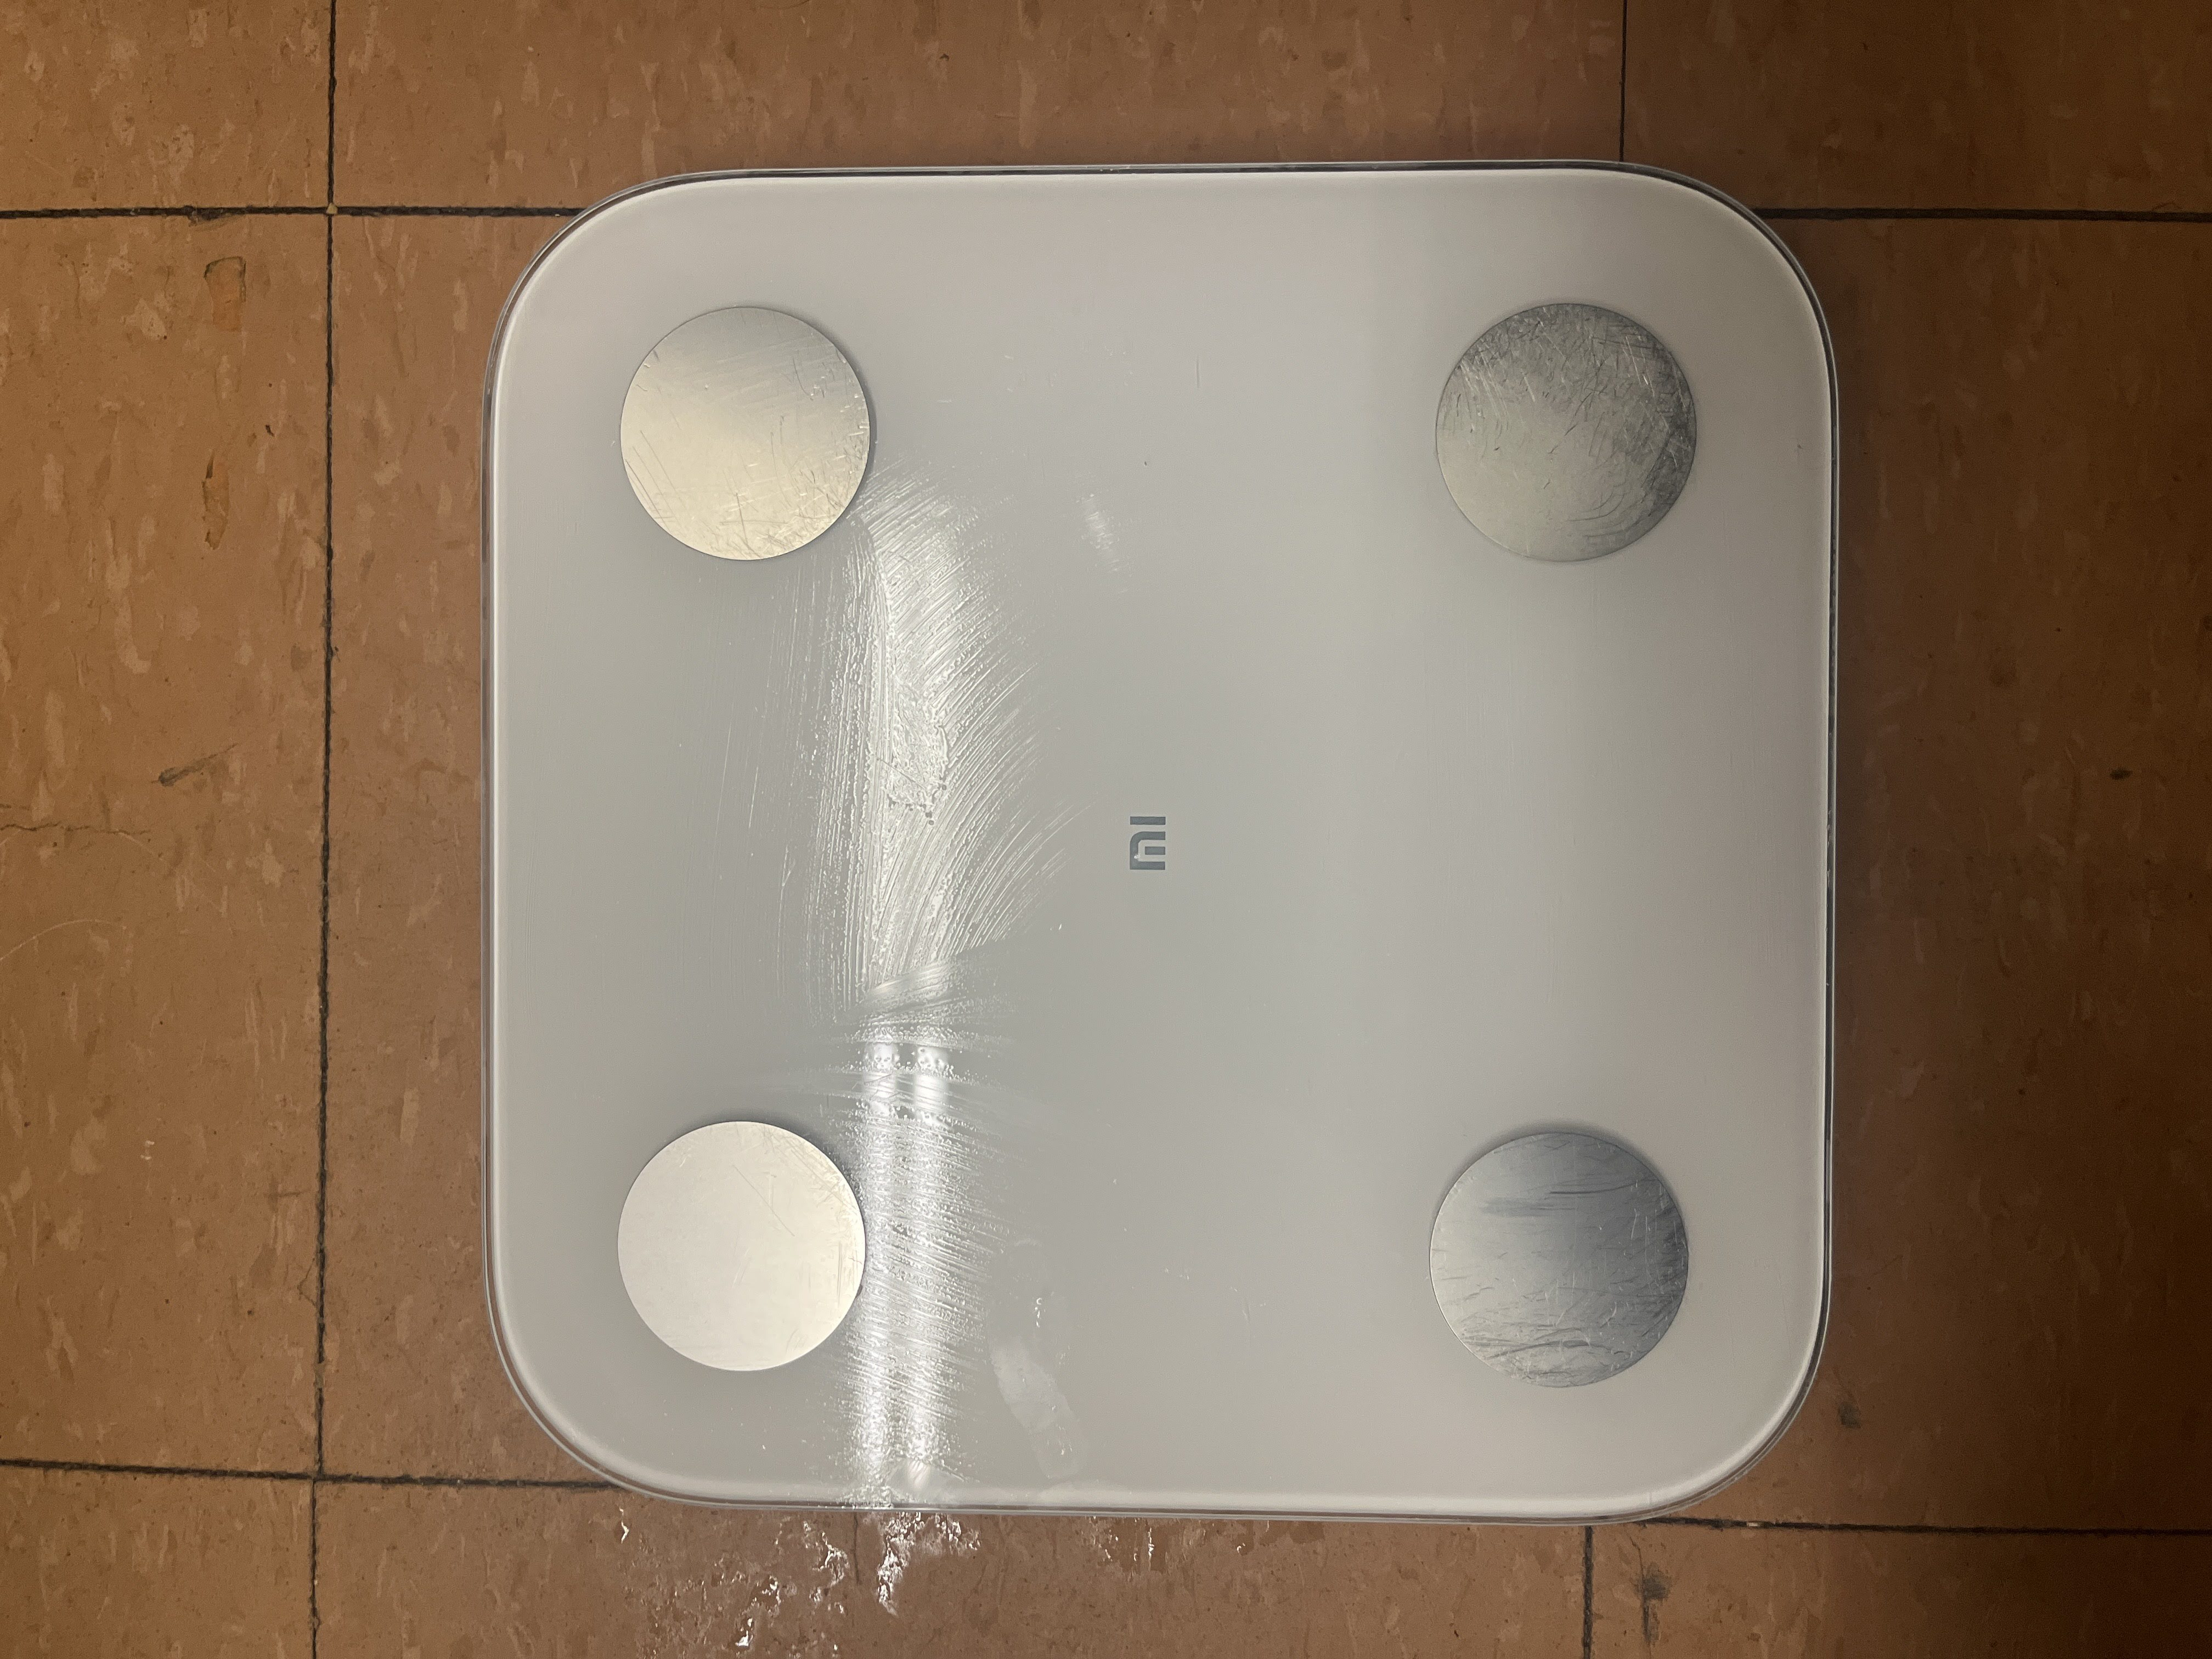
\includegraphics[width=1.7cm]{scale.jpg}
                    & 
                    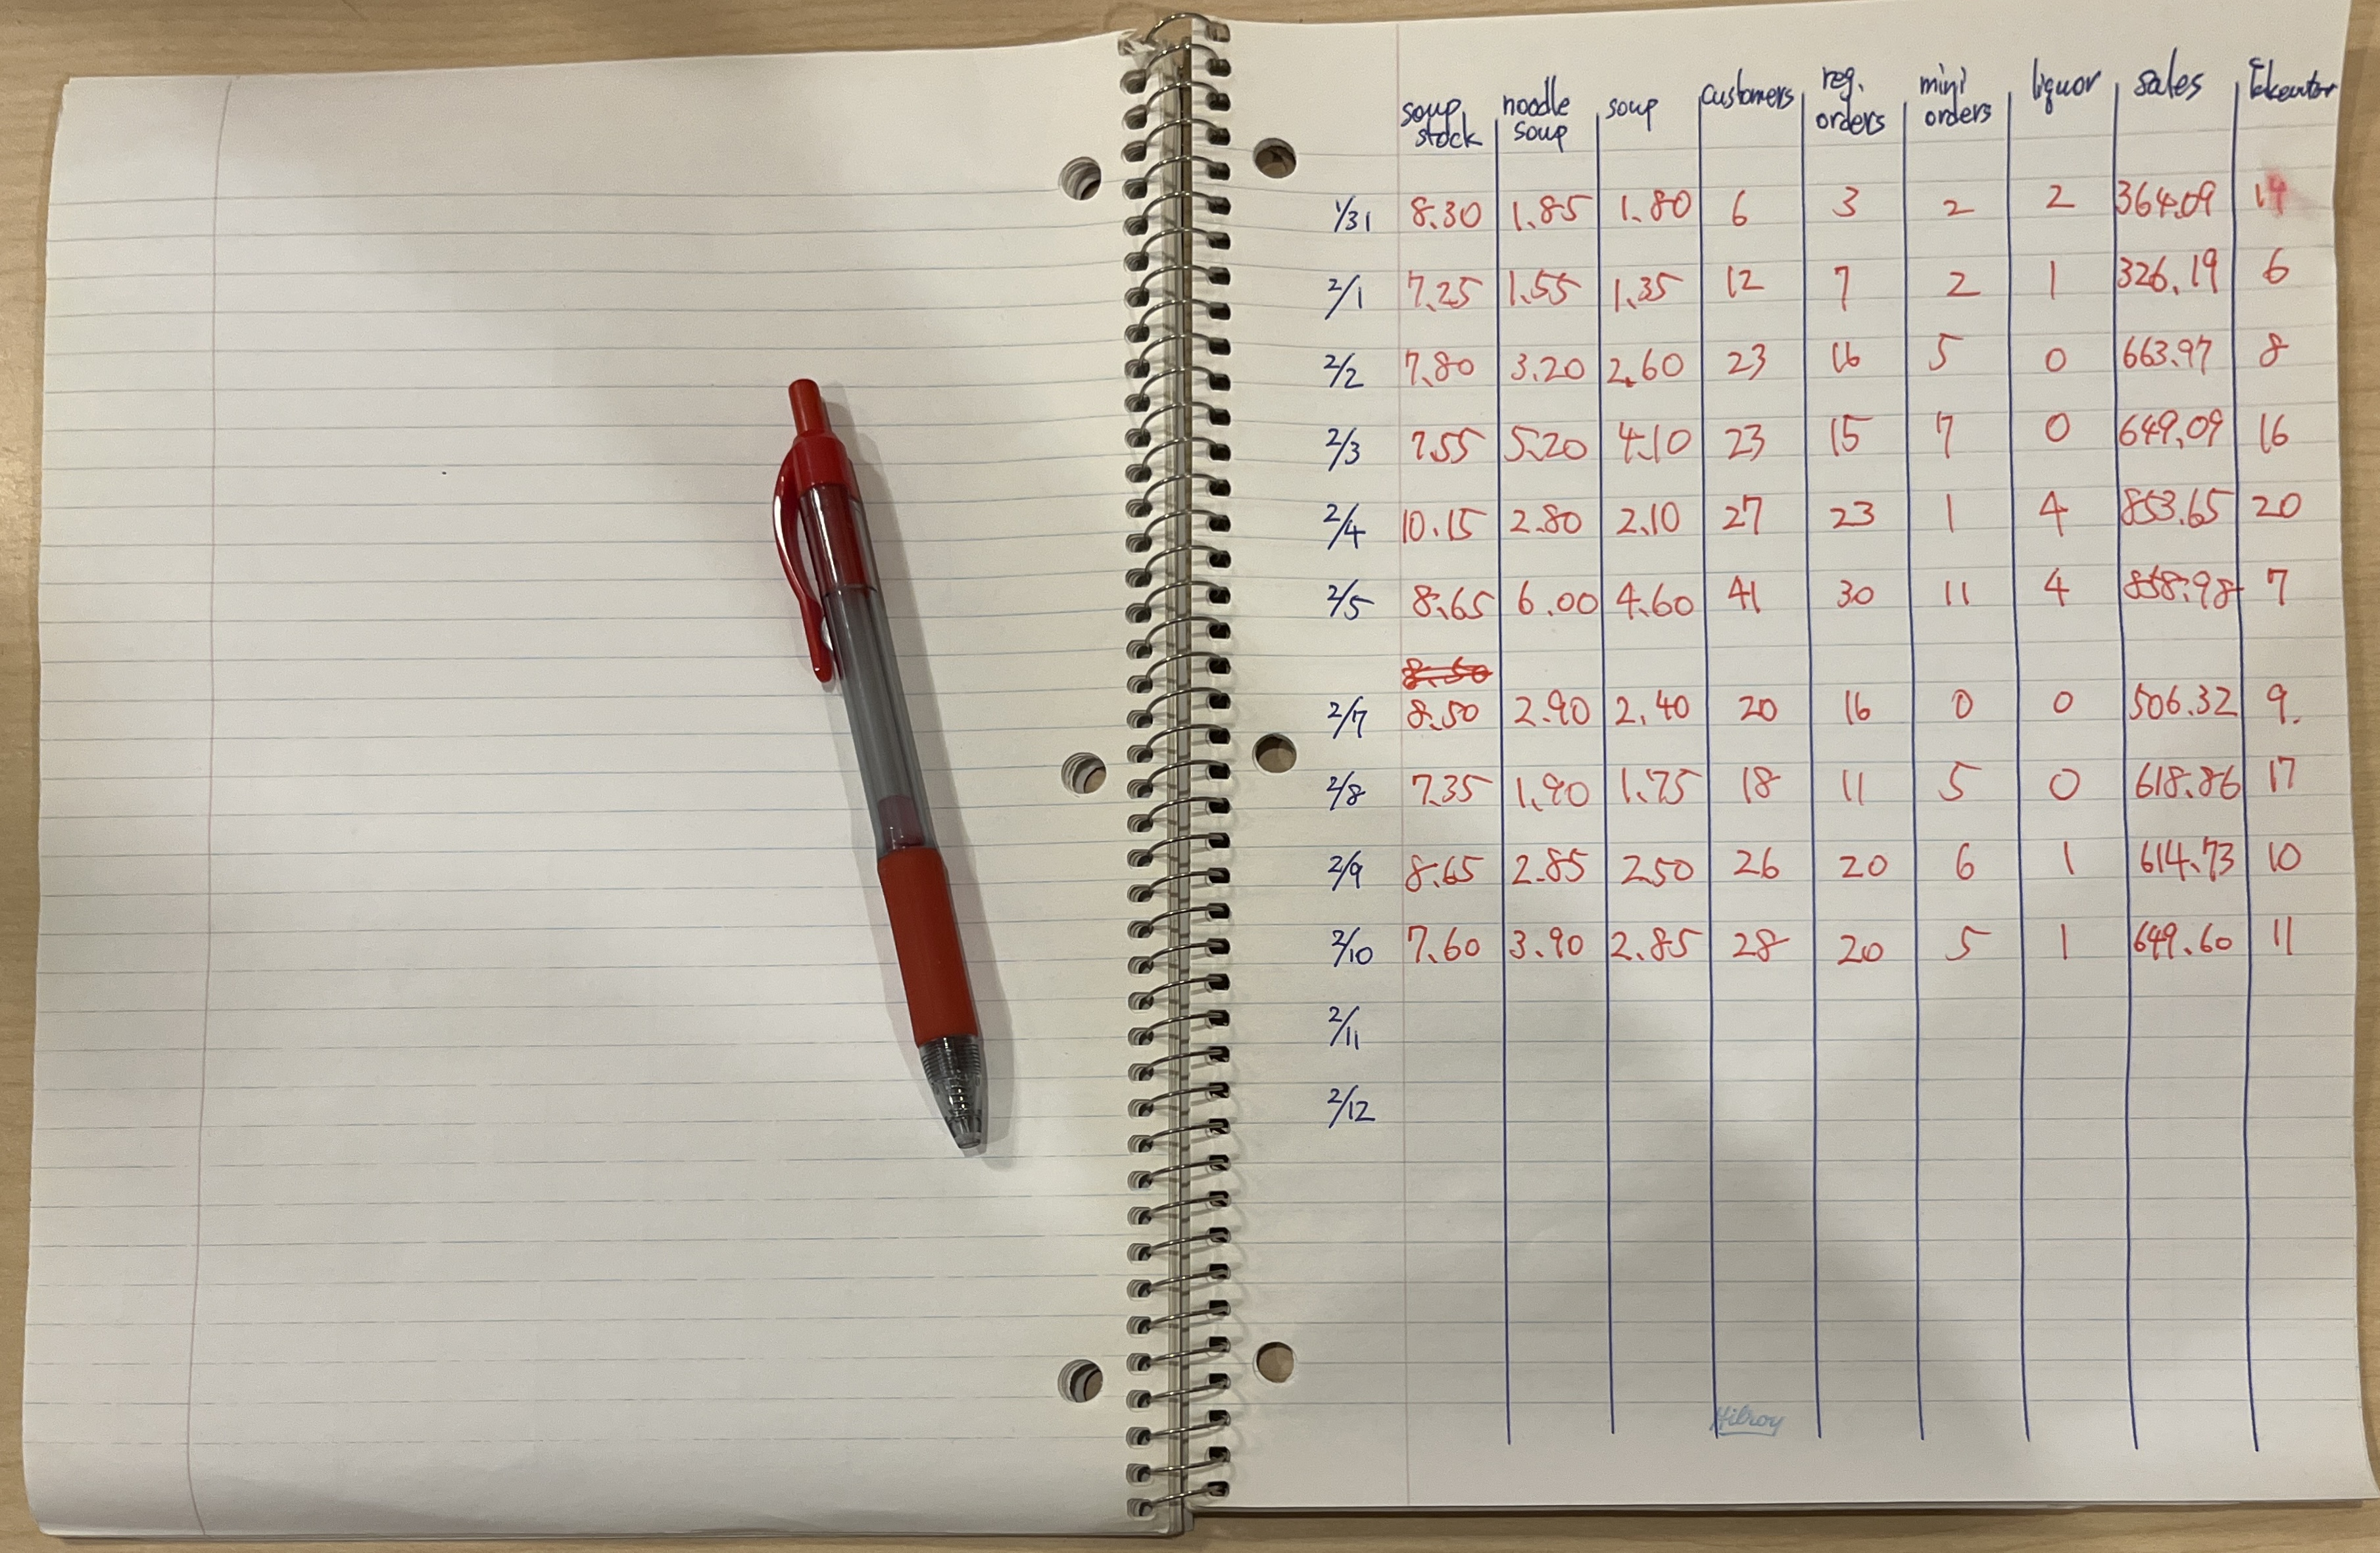
\includegraphics[width=1.7cm]{notebookPen.jpg}
                    % \hline
            \end{tabular}
            % \caption{Collection Apparatus}  
        % \end{table}  
    \end{block}
\end{frame}

% \subsection{Duration}
% \begin{frame}{Methods}
%     \underline{How many samples to be collected?}
%     \begin{block}{Sample Size}
%         \begin{itemize}
%             \item \textbf{Power analysis}, 
%             114 samples: 90\% CI and 10\% margin of error with 10 explanatory variables.
%             \item \textbf{Rule-of-thumb}, one-in-ten rule suggests 100 observations with 10 predictors\cite{Harrell1984-te}
%             \item Green's rule states 130 samples with 10 predictors\cite{Green1991-aj}
%         \end{itemize}
%     \end{block}
% \end{frame}

%%%%%%%%%%%%%%%%%%%%%%%%%%%%%%%%%%%%%%%
% Methods
%% Variables: Collect data %%
%%%%%%%%%%%%%%%%%%%%%%%%%%%%%%%%%%%%%%%
\subsection{Variables}
\begin{frame}{Methods}
    \begin{block}{Research Variables}
    \small
        \begin{tabular}{ll}
            \hline
            Variables & Note \\ \hline
            1.Food Loss & Daily disposed food by kitchen \\
            2.Liquid Food Waste & Daily disposed liquid food by customers \\
            3.Solid Food Waste & Daily disposed solid food by customers \\ \hline
            4.\# of Customers & Daily number of dine-in customers \\
            5.Sales & Daily sales \\
            6.Liquor & Daily number of liquors sold \\
            7.Orders & Daily number of orders sold \\
            8.Takeouts & Daily number of takeout sold \\
            \vspace{0.5em}
            9.Business & Changes in operations / environment\\
            
            10.Temperature & Hourly mean temperature each day \\
            11.Humidity & Hourly mean humidity \\
            \vspace{0.5em}
            12.Precipitation & Precipitation \\ 
            13.Calendar & Week of day \\ \hline
        \end{tabular}
    \end{block}
\end{frame}

%%%%%%%%%%%%%%%%%%%%%%%%%%%%%%%%%%%%%%%
% Methods
%% Statistical Model %%
%%%%%%%%%%%%%%%%%%%%%%%%%%%%%%%%%%%%%%%
\subsection{Statistical Model}
\begin{frame}{Methods}
    \small
    \begin{block}{Multiple Linear Regression (additive) Model}
        \[
        \begin{aligned}
            \small Y &=  X\beta + \epsilon, \hspace{1em}
            \epsilon \sim N(0, \sigma_y^2).
        \end{aligned}
        \]
    \end{block}
    \begin{align*}
        \small food\_waste 
        &= \beta_0^1 + \beta_1^1 * temperature + \beta_2^1 * humidity \\
        &+ \beta_3^1 * precipitation + \beta_4^1 * customer + \beta_5^1 * sales\\ 
        &+ \beta_6^1 * liquors + \beta_7^1 * takeouts 
        + \beta_{8,...,12}^1 * day + \epsilon^1.\\
        \small solid\_waste 
        &= \beta_0^2 + \beta_1^2 * temperature + \beta_2^2 * humidity \\
        &+ \beta_3^2 * precipitation + \beta_4^2 * customer + \beta_5^2 * sales\\ 
        &+ \beta_6^2 * liquors + \beta_7^2 * takeouts 
        + \beta_{8,...,12}^2 * day + \epsilon^2.
    \end{align*}
    \normalsize $\implies$ Check each confidence interval of the coefficients.
\end{frame}

%%%%%%%%%%%%%%%%%%%%%%%%%%%%%%%%%%%%%%%
% Results
%% Expected results %%
%%%%%%%%%%%%%%%%%%%%%%%%%%%%%%%%%%%%%%%
\section{Expected Results}
\begin{frame}{Expected Results}
    \begin{block}{Expected Results}
        \begin{itemize}
            \item Estimations of FLW in a restaurant.
            \item Any patterns / factor of FLW.
            \item Implications of FLW reduction.
        \end{itemize}
    \end{block}
\end{frame}

% \subsection{Current Position}
\begin{frame}{Expected Results}
    \begin{block}{Current Progress}
        \begin{itemize}
            \item From Sept.~16, five months.
            \item Collected over 140 samples.
            \item Basic analysis (Histogram, Time series plots)
            \item Finishing statistical model.
        \end{itemize}

        \begin{table}[]
            \begin{tabular}{cc}
                \hline
                    \small Food Waste per Week of Day & Food Loss and Waste Trend \\ \hline
                    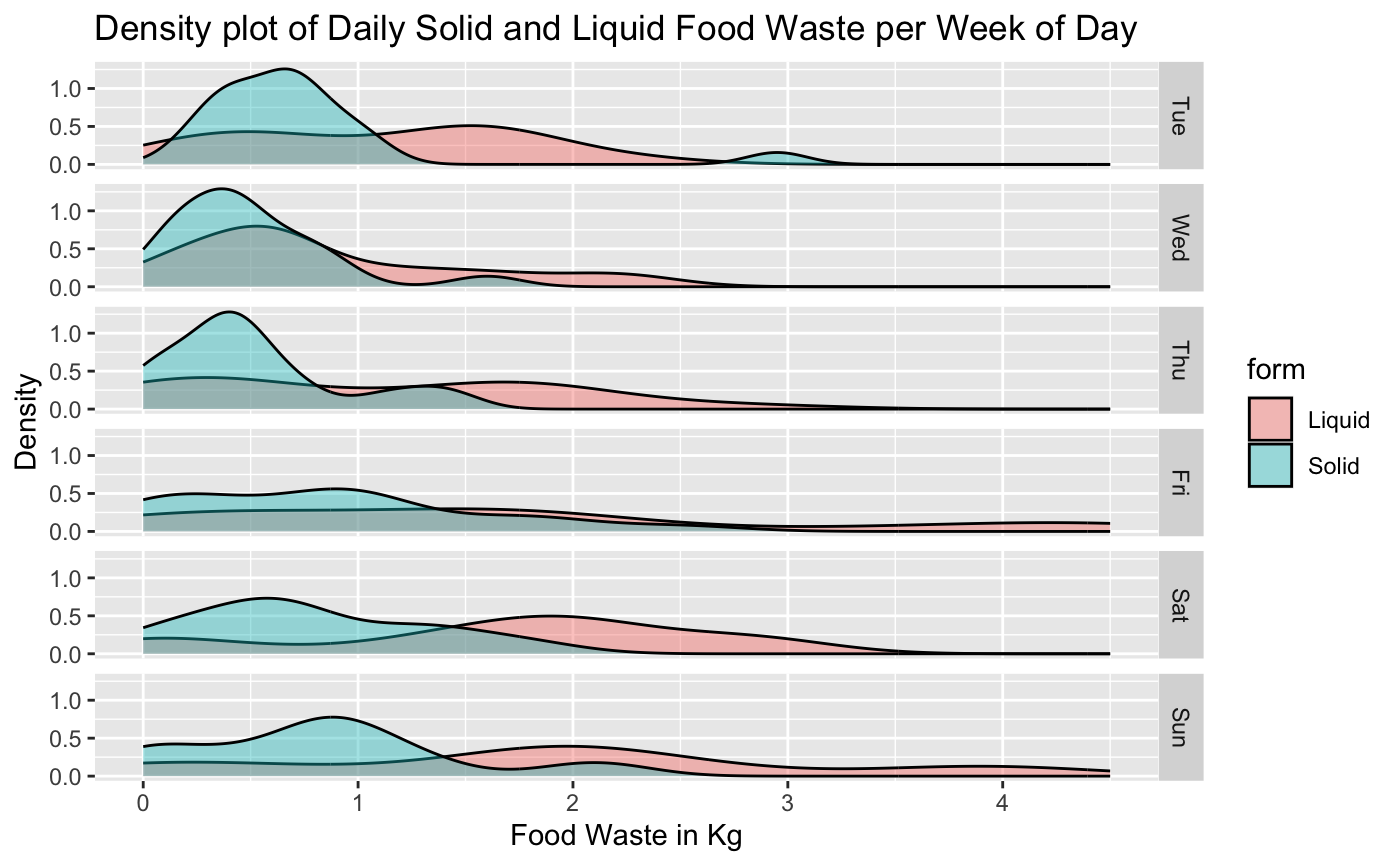
\includegraphics[width=2.2cm]{weekFW.png}
                    & 
                    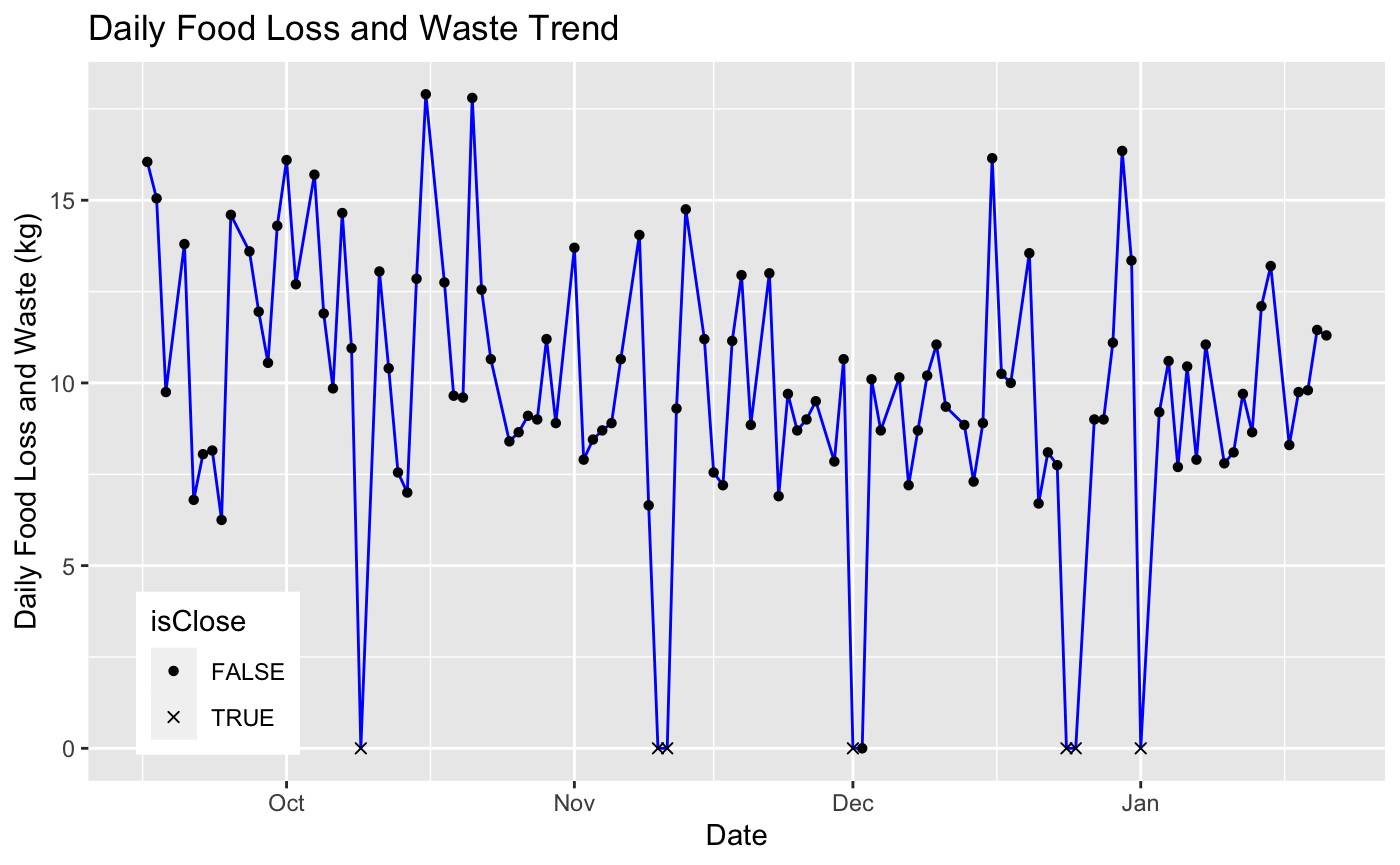
\includegraphics[width=2.5cm]{tsFLW.png}\\
                    &      \\
                \hline
            \end{tabular}
            % \caption{Sample Graphs}  
        \end{table}
    \end{block}
\end{frame}

% \subsection{Plan}
\begin{frame}{Future Plan}
    \begin{description}
        \item [September 2022 - March 2023:] Data collection
        \begin{enumerate}
            \item[1.] Mid of March: 150 samples
            \item[2.] Take photos for presentation
        \end{enumerate}
        \item [March 2023 - June 2023:] Write up of research paper.
        \begin{enumerate}
            \item[1.] Research up on potential factors: weather conditions and calendar effects.
            \item[2.] Finish up descriptive graphs and stat model, and analyze it.
            \item[3.] Explore consequence of FLW and estimate its effects
        \end{enumerate}
        \item [June - July 2023:] Prepare for thesis defence.
    \end{description}
\end{frame}

\section{Acknowledgements}
\begin{frame}{Acknowledgements}
I would like to express my gratitude to my supervisor, Dr. Balbinder Deo, and to the committee member for his support and encouragement in my initial thesis development.\\ 
I would also like to thank the University of Northern British Columbia and Prince George for allowing me an opportunity to pursue graduate studies.
\end{frame}

\begin{frame}{}
Thank you for listening to my presentation!

Any questions?
\end{frame}

\section{References}
\begin{frame}[allowframebreaks]
    \bibfont
    \printbibliography
\end{frame}

% \appendix
% \begin{frame}[fragile]{Appendix}
%     \underline{R code: sample size calculation}
%     \fontsize{6pt}{6pt}\selectfont
%     \begin{lstlisting}[language=R]
% # Single porportion test
% pwr.p.test(h=0.3, sig.level=0.05, 
%            power=0.90, alternative="two.sided")
% 
% # One Mean T-test
% pwr.t.test(d=0.3, sig.level=0.05,
%            power=0.9, type="one.sample", alternative="two.sided")
% 
% # Multiple Linear Regression
% pwr.f2.test(u=10, f2=0.15, sig.level=0.1, power=0.90)
%     \end{lstlisting}
% \end{frame}
% 
% \begin{frame}[fragile]{Appendix}
%     \underline{R code: spurious regression}
%     \fontsize{6pt}{6pt}\selectfont
%     \begin{lstlisting}[language=R]
% ## No relationship ----------------
% set.seed(1) # set rand 
% m = 0  # mean
% v = 10 # variance
% Nsample <- 400 # sample size
% 
% # simulate two sets of data
% x_sim   <- rnorm(Nsample, mean = m, sd = sqrt(v))
% y_sim   <- rnorm(Nsample, mean = m, sd = sqrt(v))
% simData <- data.frame(x = x_sim, y=y_sim)
% 
% # visualization
% autoplot(ts(simData[,c(1,2)])) # Time series
% ggplot(simData, aes(x=x,y=y)) + geom_point() # 2D scatter plot
% 
% # Linear Regression Analysis
% mod <- lm(y ~., data = simData) # fitted linear model 
% summary(mod)
% 
% ## Spurious Regression ----------------
% # generate random-walk data
% x_sim_rw   <- cumsum(rnorm(Nsample)) 
% y_sim_rw   <- cumsum(rnorm(Nsample))
% simData_rw <- data.frame(x_rw = x_sim_rw, y_rw = y_sim_rw)
% 
% autoplot(ts(simData_rw[,c(2:3)])) # Time series
% ggplot(simData_rw, aes(x=x_rw,y=y_rw)) + geom_point() # 2D scatter plot
% 
% mod <- lm(y_rw ~ x_rw, data = simData_rw)
% summary(mod)
% \end{lstlisting}
% \end{frame}
% 
% \begin{frame}[fragile]{Appendix}
%     \underline{R code: spurious regression}
%     \fontsize{6pt}{6pt}\selectfont
%     \begin{lstlisting}[language=R]
% # 100 simulations (correct p-value) ----------------
% Nsim <- 100 # Number of simulation runs
% pValues     <- numeric(Nsim) # Set vectors
% pValuesRW   <- numeric(Nsim) # Set vectors for random walk
% pValueARIMA <- numeric(Nsim) # Set vectors for ARIMA sim
% 
% # Nsim times simulation data 
% for(i in 1:Nsim){ 
%   # No random walk process
%   y <- rnorm(Nsample, sd = sqrt(v))
%   x <- rnorm(Nsample, sd = sqrt(v))
%   
%   # Random walk simulation data
%   y_rw <- cumsum(rnorm(n=Nsample))
%   x_rw <- cumsum(rnorm(n=Nsample))
%   
%   # ARIMA simulation data
%   x_arima <- arima.sim(list(order=c(2,1,1), ar=c(0.2,-0.1),# ARIMA(2,1,1)  
%                             ma=-0.1), n=Nsample) 
%   y_arima <- arima.sim(list(order=c(0,1,1), ma=0.2), n=Nsample)#ARIMA(0,1,1)
%                             
%   mod       <- lm(y ~ x) # linear regression analysis
%   mod_rw    <- lm(y_rw ~ x_rw) # linear regression analysis for rw
%   mod_arima <- lm(y_arima ~ x_arima) # linear regression analysis for arima
%   
%   # Save p-value
%   pValues[i]     <- summary(mod)$coefficients[2,4]
%   pValuesRW[i]   <- summary(mod_rw)$coefficients[2,4]
%   pValueARIMA[i] <- summary(mod_arima)$coefficients[2,4]
% }
%     \end{lstlisting}
% \end{frame}
% 
% \begin{frame}[fragile]{Appendix}
%     \underline{R code: spurious regression}
%     \fontsize{6pt}{6pt}\selectfont
%     \begin{lstlisting}[language=R]
% # Combine data 
% simPresult <- data.frame(pValues = c(pValues, pValuesRW, pValueARIMA),
%                          simPattern = rep(c("Regression", 
%                                             "Regression of RW",
%                                             "Regression of ARIMA"), 
%                                           each = Nsim))
% 
% # Histograms
% histPlot <- 
%   ggplot(simPresult, aes(x = pValues, fill = simPattern)) + 
%   geom_histogram(alpha = 0.5, position = "identity", binwidth  = 0.1)
% plot(histPlot)
%     \end{lstlisting}
% \end{frame}
% 
% \begin{frame}[fragile]{Appendix}
%     \underline{Stan code: dynamic linear regression}
%     \fontsize{6pt}{6pt}\selectfont
%     \begin{lstlisting}[language=R]
% data{
%   int T;       // Number of observations
%   vector[T] x; // explanatory variable
%   vector[T] y; // response variable
% }
% parameters{
%   vector[T] a;       // intercepts
%   vector[T] b;       // coefficient
%   real<lower=0> s_a; // s.d. for intercept
%   real<lower=0> s_b; // s.d. for coefficient
%   real<lower=0> s_mu;// s.d. for estimated state
% }
% transformed parameters {
%   vector[T] mu;   // estimations of state each observed time
%   
%   for(i in 1:T) { // mu = a + b * x for each time
%     mu[i] = a[i] + b[i] * x[i];
%   }
% }
% model {
%   for(i in 2:T) {  // State transitioned as per the state equation
%     a[i] ~ normal(a[i-1], s_a); // a_i = a_{i-1} + N(0,s_a)
%     b[i] ~ normal(b[i-1], s_b); // b_i = b_{i-1} + N(0,s_b)
%   }
%   // Observations are obtained per the given observation equation
%   for(i in 1:T){
%     y[i] ~ normal(mu[i], s_mu);
%   }
% }
%     \end{lstlisting}
% \end{frame}

\end{document}
